\documentclass{article}
\usepackage[utf8]{inputenc}
\usepackage{capt-of} % Für captionof
\usepackage{hyperref} % Für Links

\title{Macherdaach-Badge \\ Lötanleitung \\ [1cm]
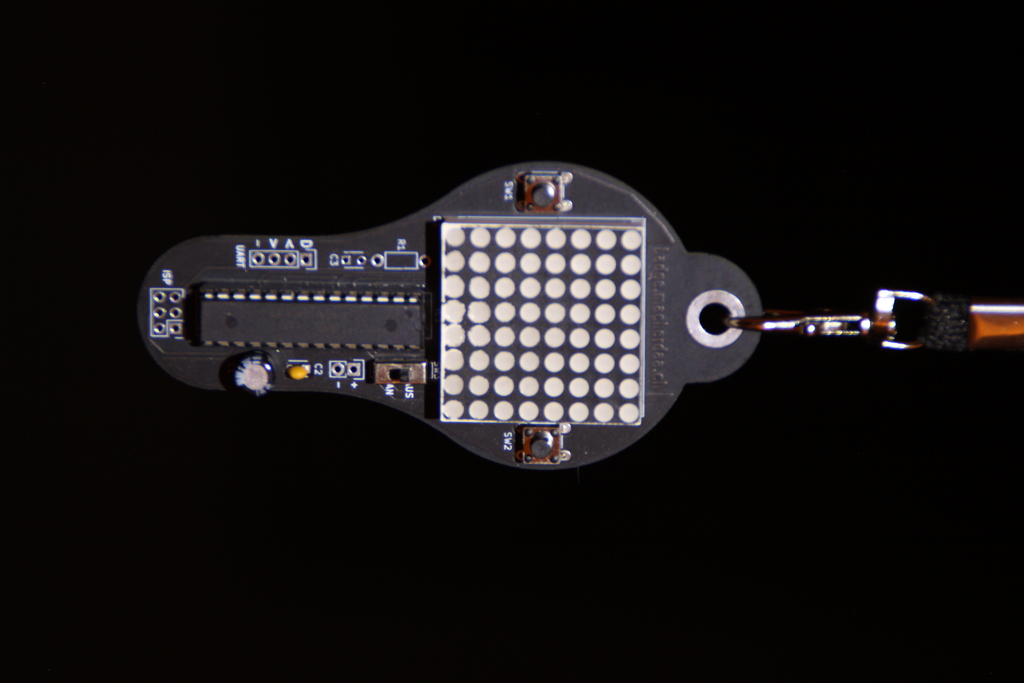
\includegraphics[width=0.7\textwidth, angle=90]{Bilder2022/IMG_8263.JPG}
}
\date{September 2022}
\author{casartar\\casartar@web.de}

\usepackage{natbib}
\usepackage{graphicx}
\usepackage[ngerman]{babel} % Macht aus Figure -> Abbildung

\setlength{\parindent}{0pt} % Keine Einrückung nach Absatz

\usepackage{geometry} % Seitenränder ein bisschen schmaler
\geometry{
  left=2cm,
  right=2cm,
  top=2cm,
  bottom=2cm,
  bindingoffset=5mm
}

\begin{document}

\maketitle
\newpage
\section{Einleitung}

Das Macherdaach-Badge ist ein kleiner Bausatz zum selber zusammenlöten, der extra für den Landauer Maker Day entwickelt wurde.
Du musst nur wenige Bauteile verlöten, bis du ein vollfunktionsfähes Badge dein Eigen nennen darfst. Neben coolen Mustern und einem Minispiel, wird in jedes Badge eine individuelle Laufschrift nur für dich einprogrammiert.\\

Wir wünschen viel Spaß und gutes Gelingen. 

\section{Die Bauteile stellen sich vor}
Alle Bauteile, die du für deinen Macherdaach-Badge brauchst, findest du in einer Tüte, die du von einem der freundlichen Helfer am Tisch überreicht bekommst.

Folgende Bauteile sollten in der Tüte drin sein:

\begin{enumerate}
	\item Macherdaach Badge Platine
	\item LED-Matrix
	\item Sockel für den Mikrocontroller
	\item Zwei Taster
	\item 100 nF Kondensator
	\item 100 $\mu$F Elektrolytkondensator
	\item Schiebeschalter
	\item Knopfzellenhalter
	\item Knopfzelle
\end{enumerate}

Den Mikrocontroller bekommst du nach dem Löten an der Programmierstation.

\newpage

\begin{center}
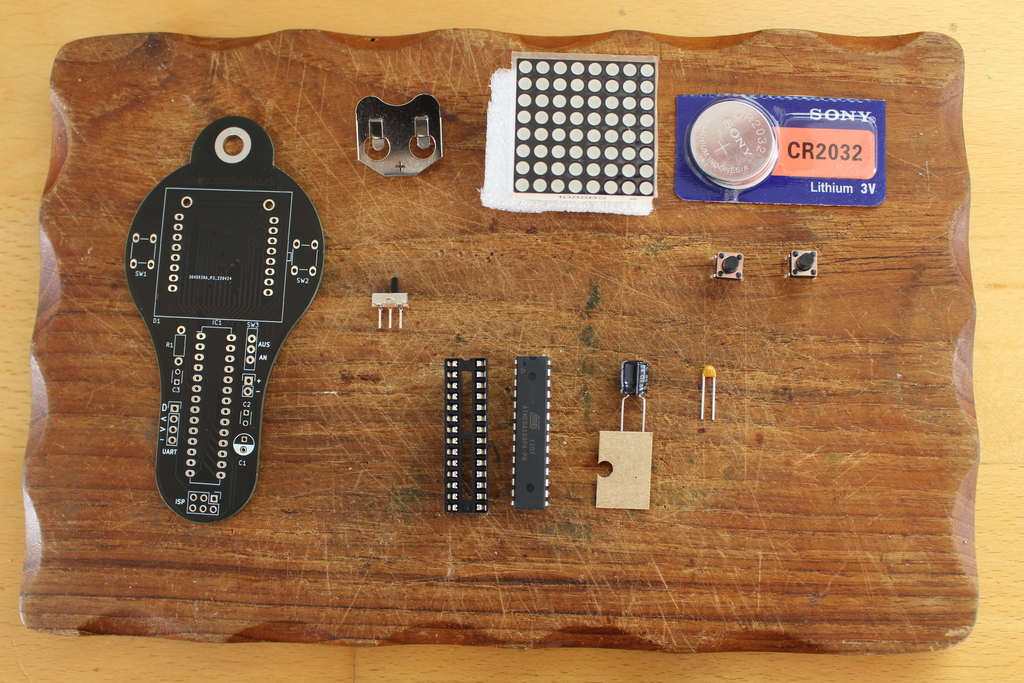
\includegraphics[width=\textwidth]{Bilder2022/IMG_8183.JPG}
\captionof{figure}{Alle Bauteile auf einen Blick}
\label{fig:all_components}
\end{center}

\section{Dokumentation ist alles}

Die Hardware, Software und selbstverständlich diese Anleitung sind Open Source. Wenn du sie dir ansehen, sie herunterladen oder daran mitarbeiten möchtest, musst du nur folgenden Links folgen:

\begin{itemize}
	\item \url{https://github.com/casartar/MacherDaachBadgeFirmware}
	\item \url{https://github.com/casartar/MacherDaachBadgeHardware}
	\item \url{https://github.com/casartar/MacherDaachBadgeDoku}
\end{itemize}

Oder suche auf github.com nach Macherdaach.

\section{Jetzt geht es richtig los}
Wir löten die Bauteile nach der Regel: Das niedrigste Bauteil zuerst.

\subsection{Kondensatoren - C2 (100 nF)}

Zuerst nimmst du den 100 nF Kondensator und steckst ihn an die mit C2 markierte Stelle auf der Platine.
Dann legst du die Platine so hin, dass der Kondensator gegen das Brett gedrückt wird und verlötest die beiden Beinchen.
Zum Schluss müssen die überstehenden Beinchen noch mit der Zange abgezwickt werden.

\vspace{1cm}

\begin{minipage}[b]{0.5\textwidth}
	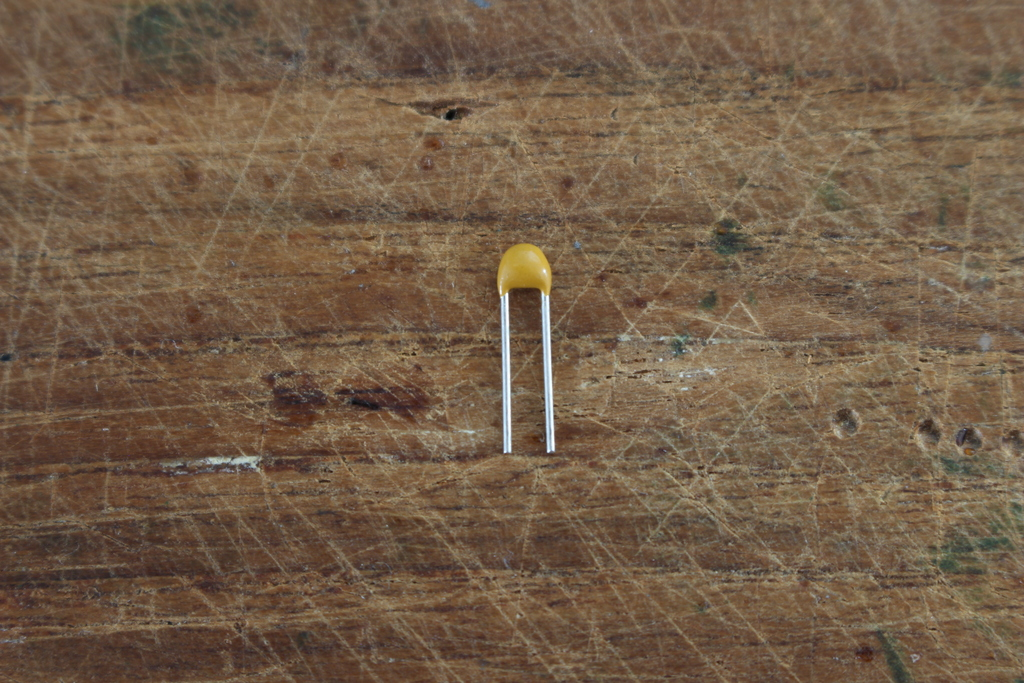
\includegraphics[width=\textwidth]{Bilder2022/IMG_8185.JPG}
	%\captionof{figure}{}
	%\label{fig:}
\end{minipage}
\begin{minipage}[b]{0.5\textwidth}
	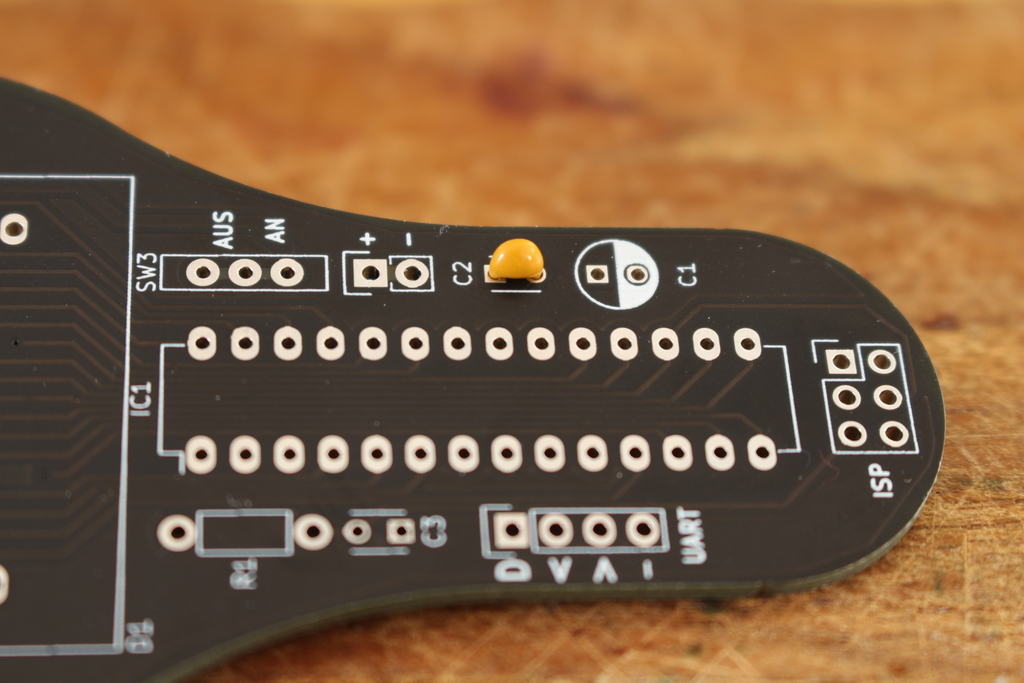
\includegraphics[width=\textwidth]{Bilder2022/IMG_8186.JPG}
	%\captionof{figure}{}
	%\label{fig:}
\end{minipage}

\vspace{0.5cm}

\begin{minipage}[b]{0.5\textwidth}
	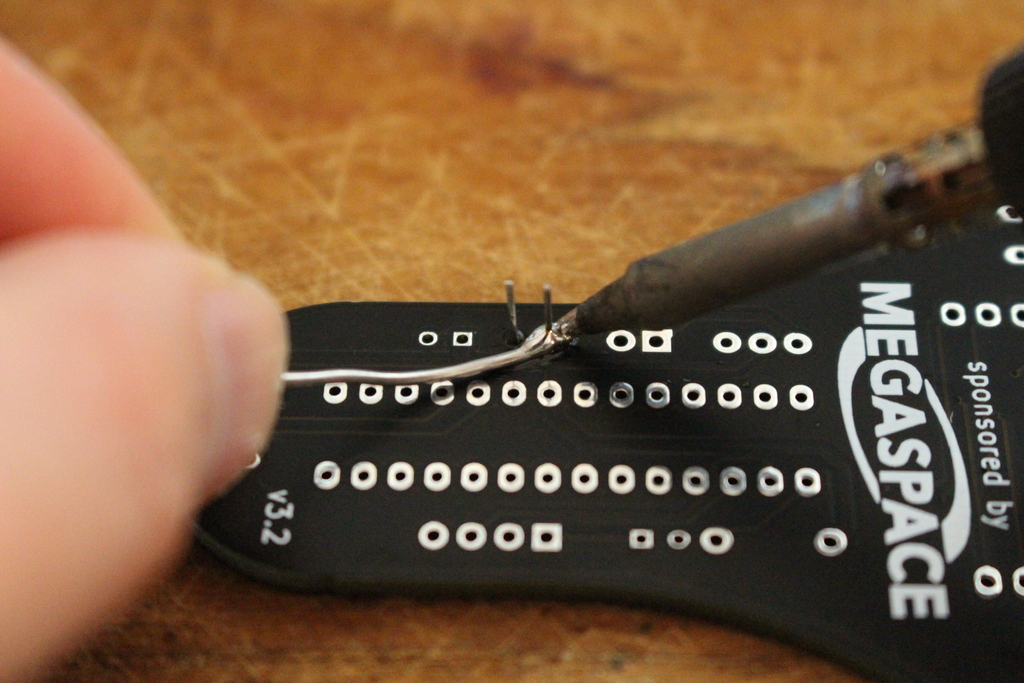
\includegraphics[width=\textwidth]{Bilder2022/IMG_8194.JPG}
	%\captionof{figure}{}
	%\label{fig:}
\end{minipage}
\begin{minipage}[b]{0.5\textwidth}
	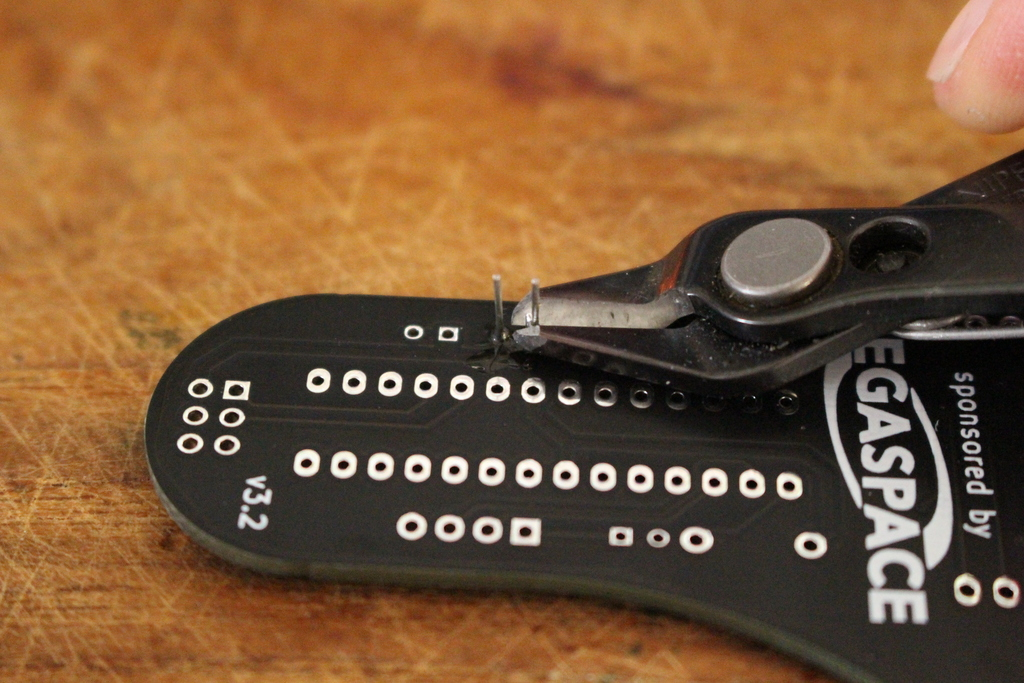
\includegraphics[width=\textwidth]{Bilder2022/IMG_8195.JPG}
	%\captionof{figure}{}
	%\label{fig:}
\end{minipage}

\vspace{0.5cm}

\subsection{Sockel für den Mikrocontroller}

Beim Sockel musst du ein bisschen aufpassen, dass er richtigherum eingelötet wird. Wenn er falschrum drin ist, ist das zwar kein Beinbruch, aber beim Löten von Platinen sollte man immer eine gewisse Sorgfalt walten lassen und auch auf solche Details achten.

Der Sockel hat eine halbrunde Einkerbung auf der einen Seite. Diese muss an der Seite auf der Platine platziert werden, wo die Pin 1 Markierung des Mikrocontrollers aufgedruckt ist. Die Markierung ist ein kleiner Querstrich links unterhalb der IC1 Beschriftung.

Wenn der Sockel richtig sitzt, kannst du die Platine wieder umdrehen und die Platine mit dem Sockel gegen das Brett drücken. Dann verlötest du am besten einen Pin und prüfst noch einmal, ob der Sockel auch wirklich richtig auf der Platine aufsitzt. Ist alles okay, kannst du alle anderen Pins in einem Rutsch festlöten.

\vspace{1cm}

\begin{minipage}[b]{0.5\textwidth}
	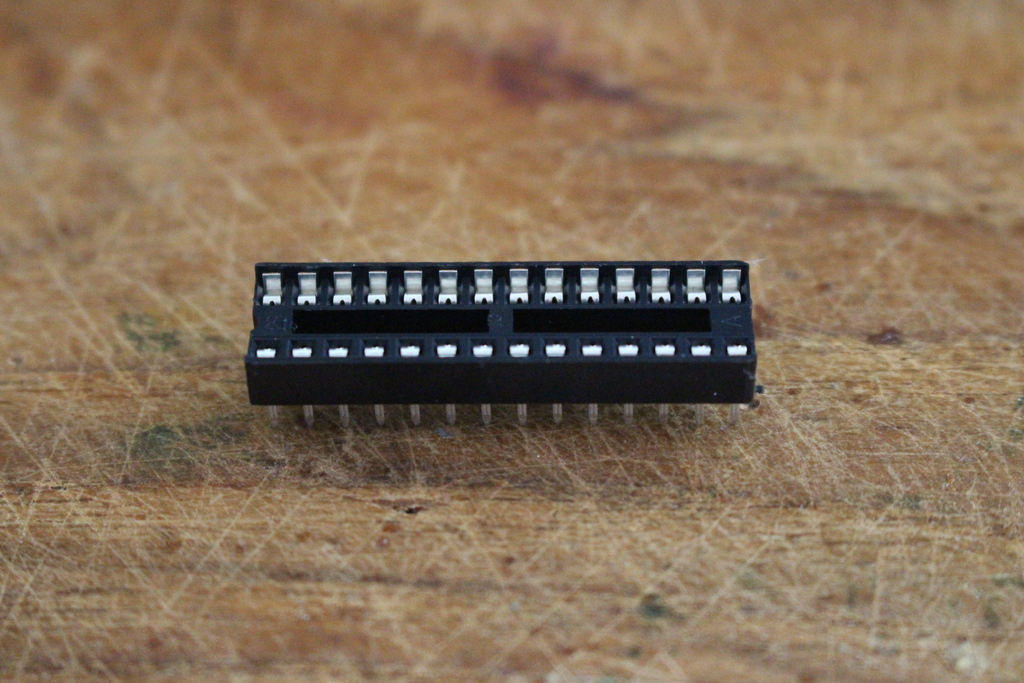
\includegraphics[width=\textwidth]{Bilder2022/IMG_8196.JPG}
	%\captionof{figure}{}
	%\label{fig:}
\end{minipage}
\begin{minipage}[b]{0.5\textwidth}
	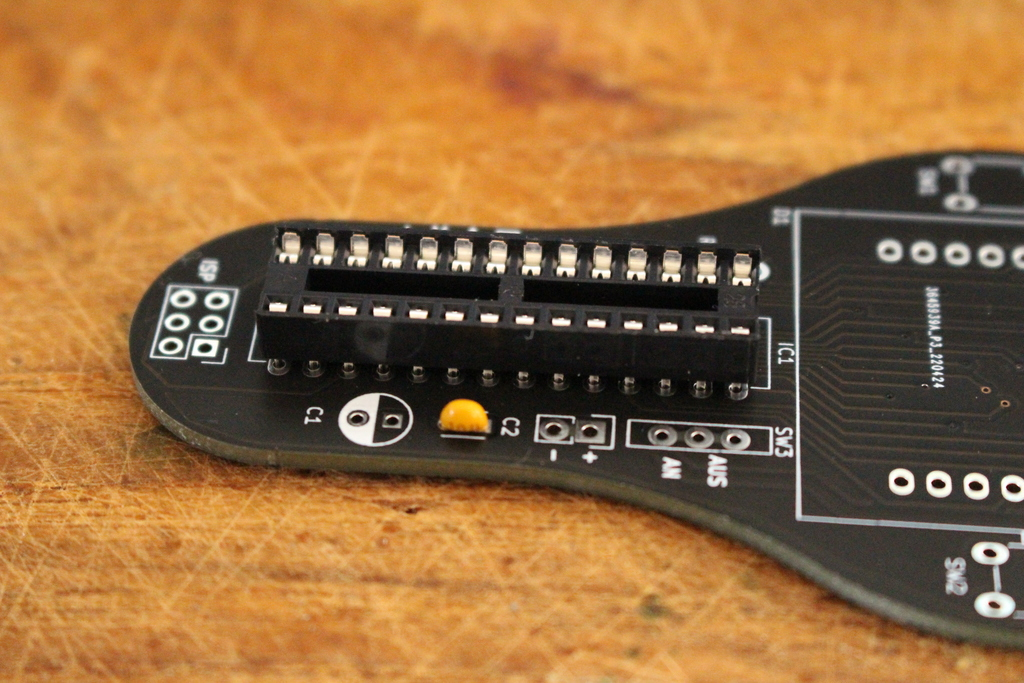
\includegraphics[width=\textwidth]{Bilder2022/IMG_8197.JPG}
	%\captionof{figure}{}
	%\label{fig:}
\end{minipage}

\vspace{0.5cm}

\begin{minipage}[b]{0.5\textwidth}
	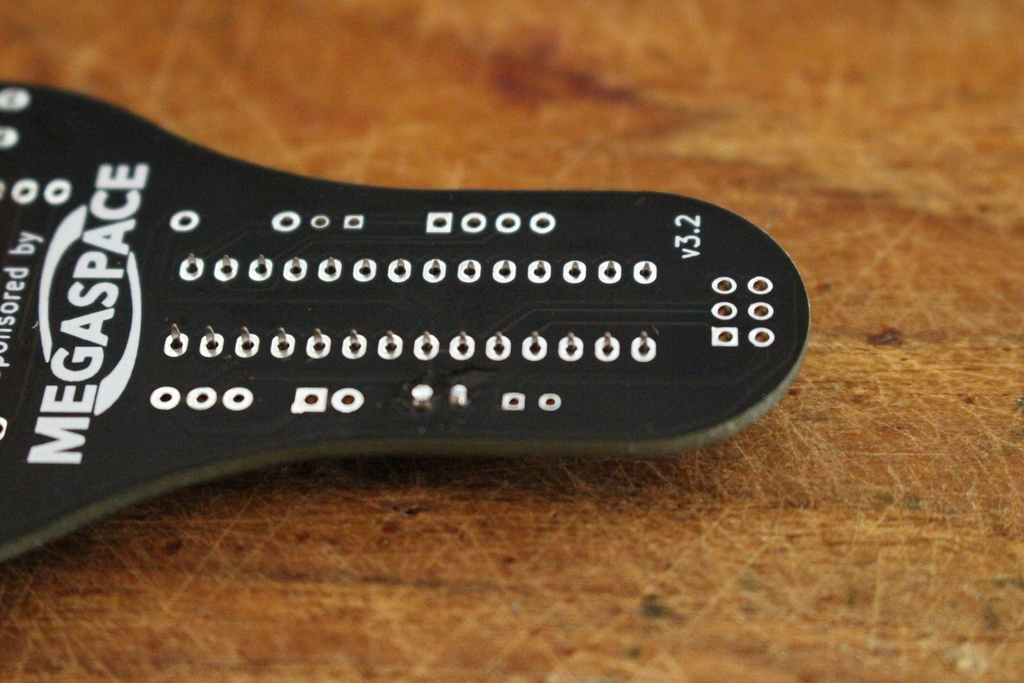
\includegraphics[width=\textwidth]{Bilder2022/IMG_8198.JPG}
	%\captionof{figure}{}
	%\label{fig:}
\end{minipage}
\begin{minipage}[b]{0.5\textwidth}
	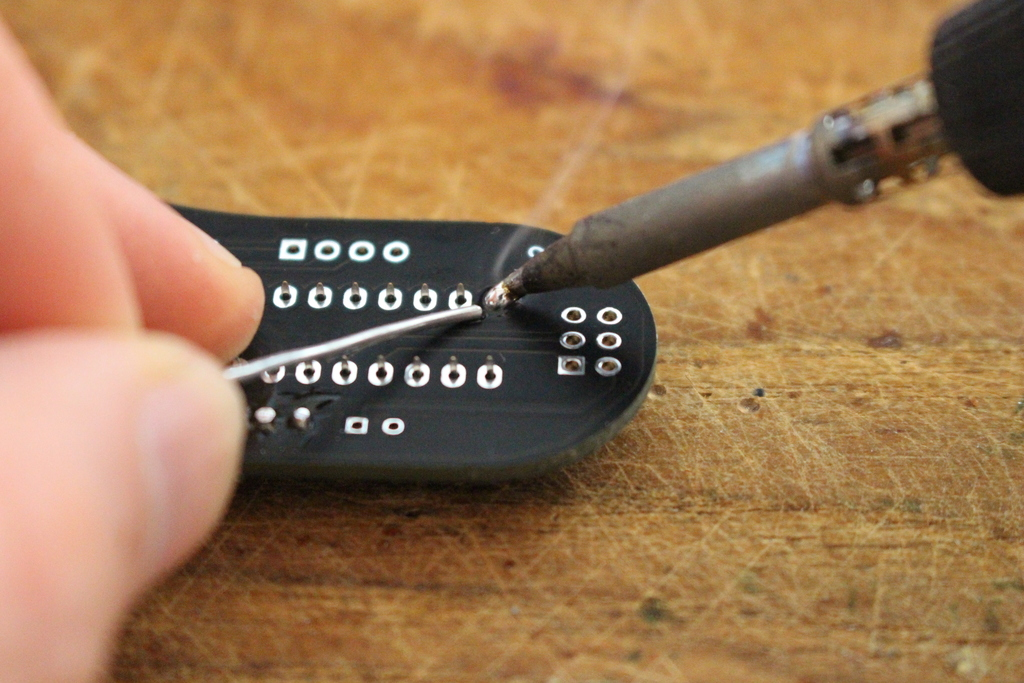
\includegraphics[width=\textwidth]{Bilder2022/IMG_8199.JPG}
	%\captionof{figure}{}
	%\label{fig:}
\end{minipage}

\vspace{0.5cm}

\begin{minipage}[b]{0.5\textwidth}
	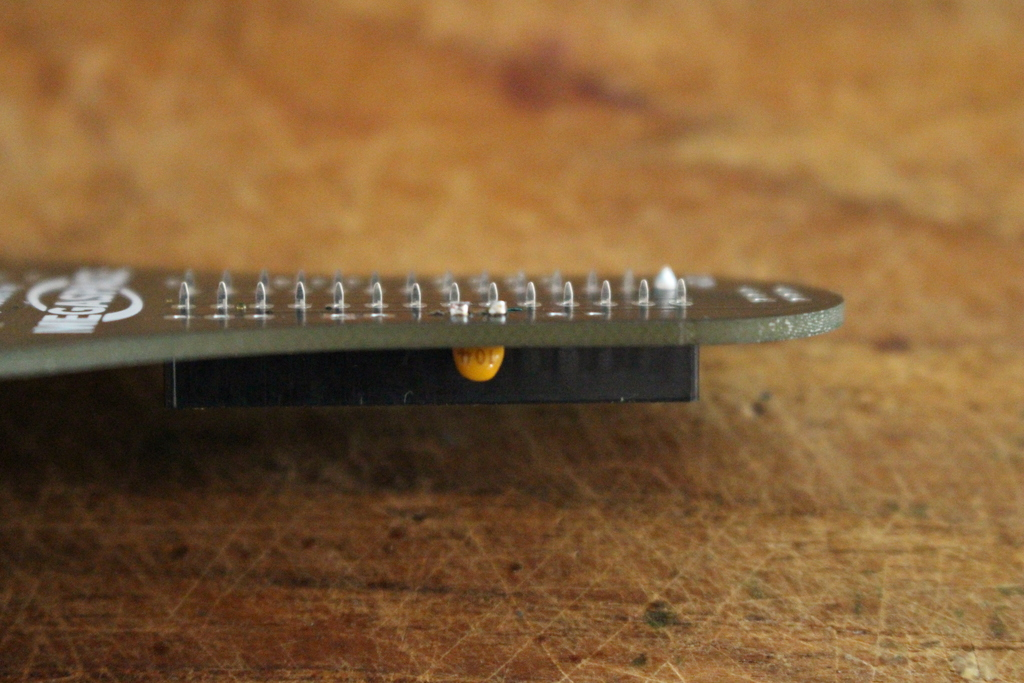
\includegraphics[width=\textwidth]{Bilder2022/IMG_8200.JPG}
	%\captionof{figure}{}
	%\label{fig:}
\end{minipage}

\subsection{Knopfzellenhalter - BT1}

Bevor du den Knopfzellenhalter anlöten darfst, musst du die große runde silberne Fläche mit Lötzinn versehen. Dazu lässt du ein kleines bisschen Lötzinn auf der Fläche schmelzen und verteilst sie mit dem Lötkolben, indem du den Lötkolben kreisförmig über die Fläche bewegst.

Das musst du tun, damit die Knopfzelle später einen ordentlichen Kontakt zur Platinenoberfläche hat.

Wenn du den Knopfzellenhalter festlötest, wirst du merken, dass das nicht so einfach geht, wie bei den Pins vorher. Das liegt daran, dass das viele Metall des Halters länger braucht um warm zu werden. Hier musst du also nur ein bisschen Geduld haben, bis das Lötzinn ordentlich fließt.

\vspace{1cm}

\begin{minipage}[b]{0.5\textwidth}
	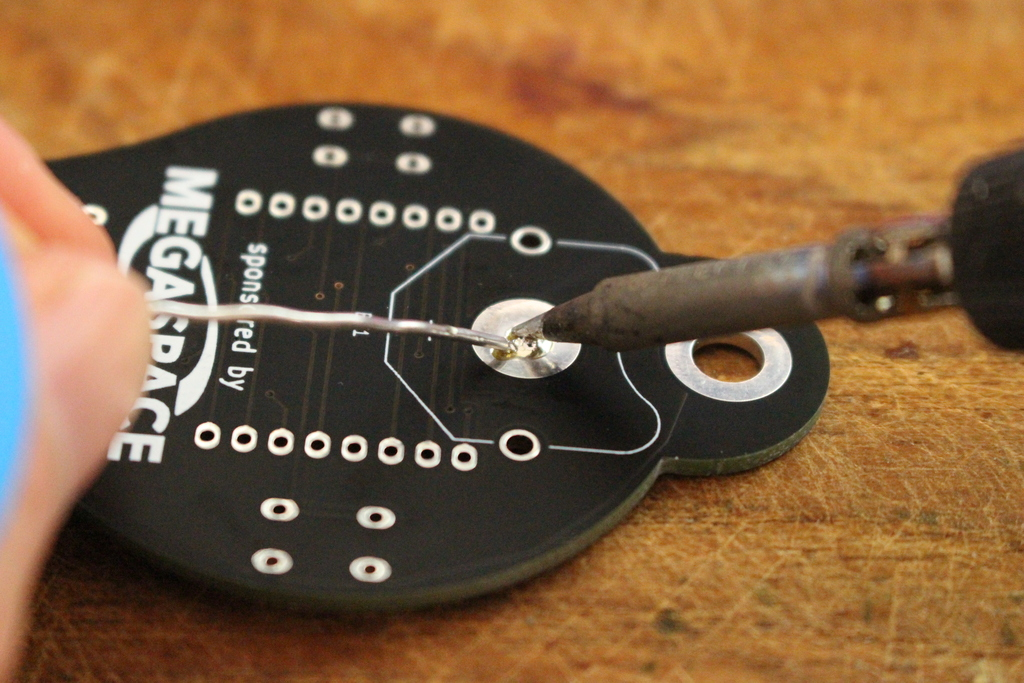
\includegraphics[width=\textwidth]{Bilder2022/IMG_8202.JPG}
	%\captionof{figure}{}
	%\label{fig:}
\end{minipage}
\begin{minipage}[b]{0.5\textwidth}
	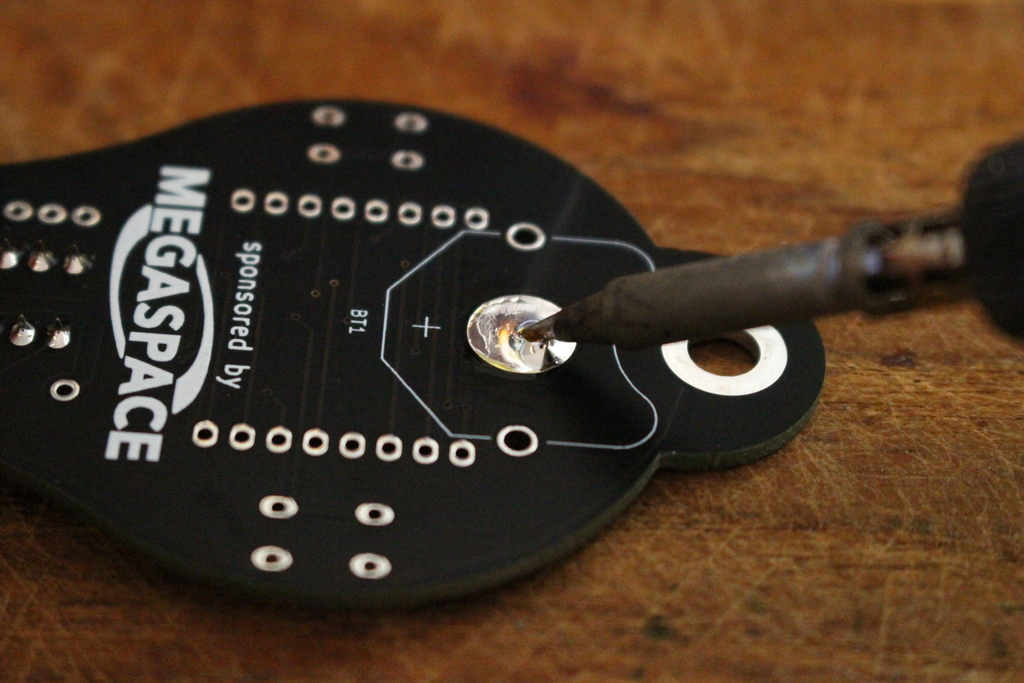
\includegraphics[width=\textwidth]{Bilder2022/IMG_8203.JPG}
	%\captionof{figure}{}
	%\label{fig:}
\end{minipage}

\vspace{0.5cm}

\begin{minipage}[b]{0.5\textwidth}
	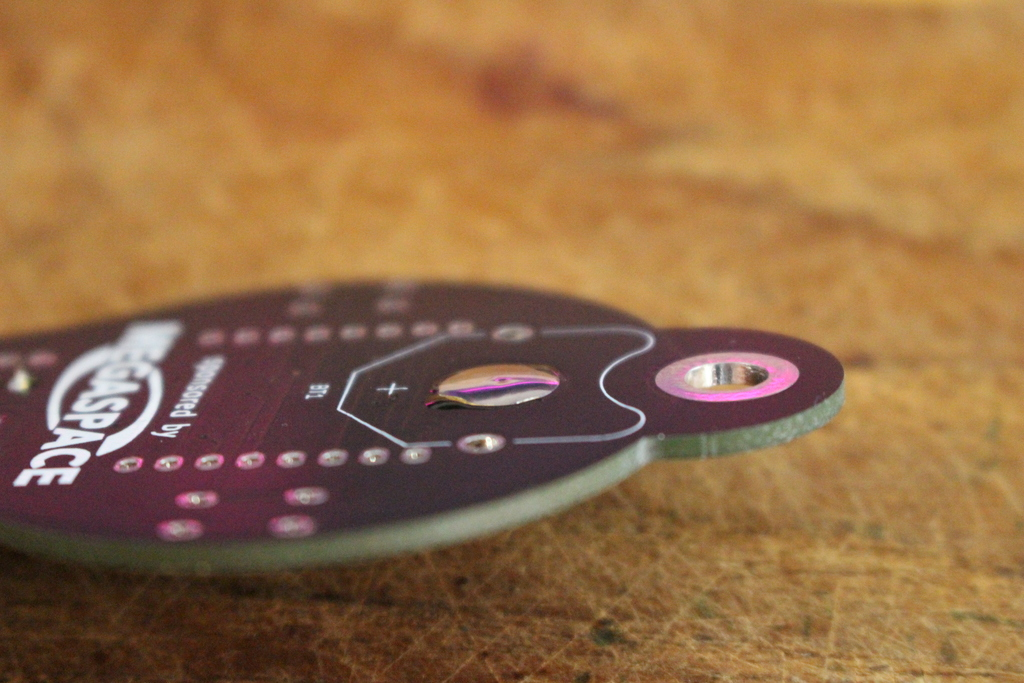
\includegraphics[width=\textwidth]{Bilder2022/IMG_8207.JPG}
	%\captionof{figure}{}
	%\label{fig:}
\end{minipage}
\begin{minipage}[b]{0.5\textwidth}
	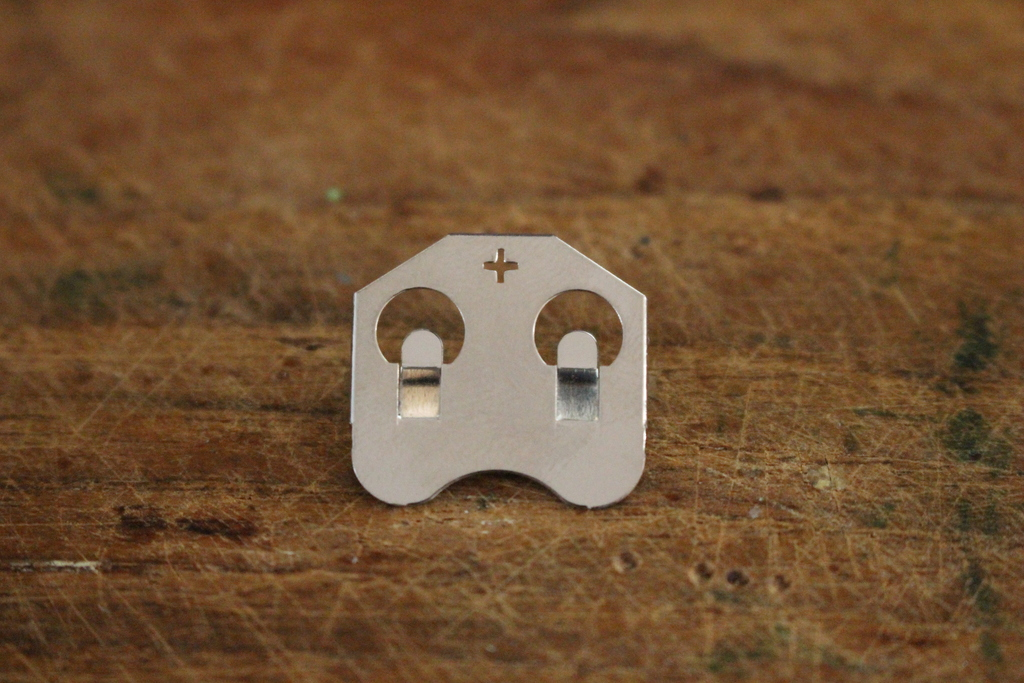
\includegraphics[width=\textwidth]{Bilder2022/IMG_8208.JPG}
	%\captionof{figure}{}
	%\label{fig:}
\end{minipage}

\vspace{0.5cm}

\begin{minipage}[b]{0.5\textwidth}
	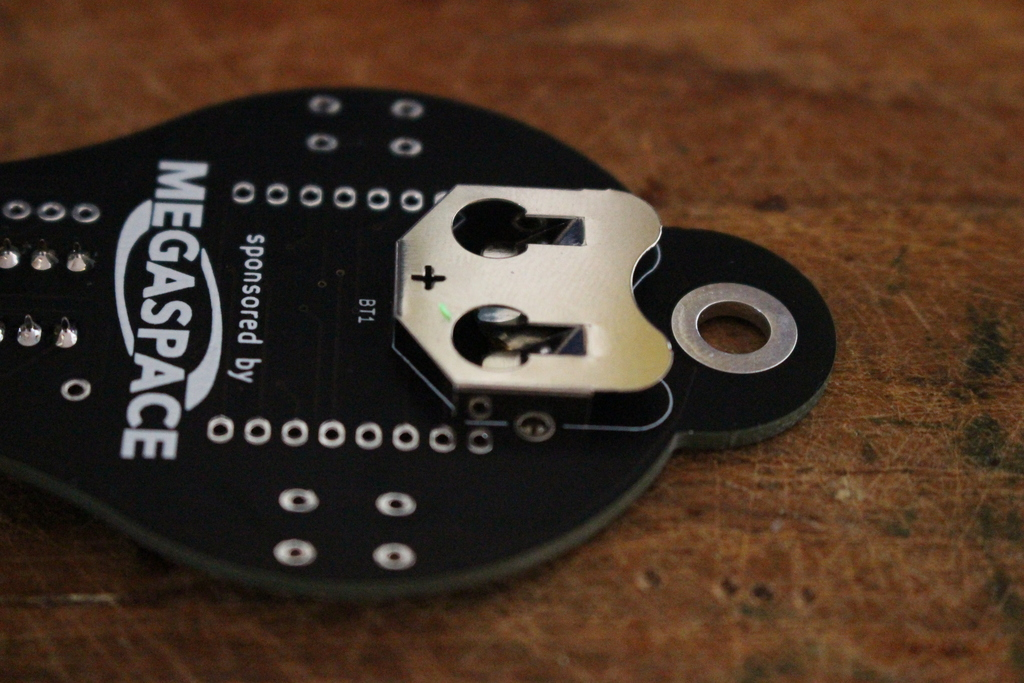
\includegraphics[width=\textwidth]{Bilder2022/IMG_8209.JPG}
	%\captionof{figure}{}
	%\label{fig:}
\end{minipage}
\begin{minipage}[b]{0.5\textwidth}
	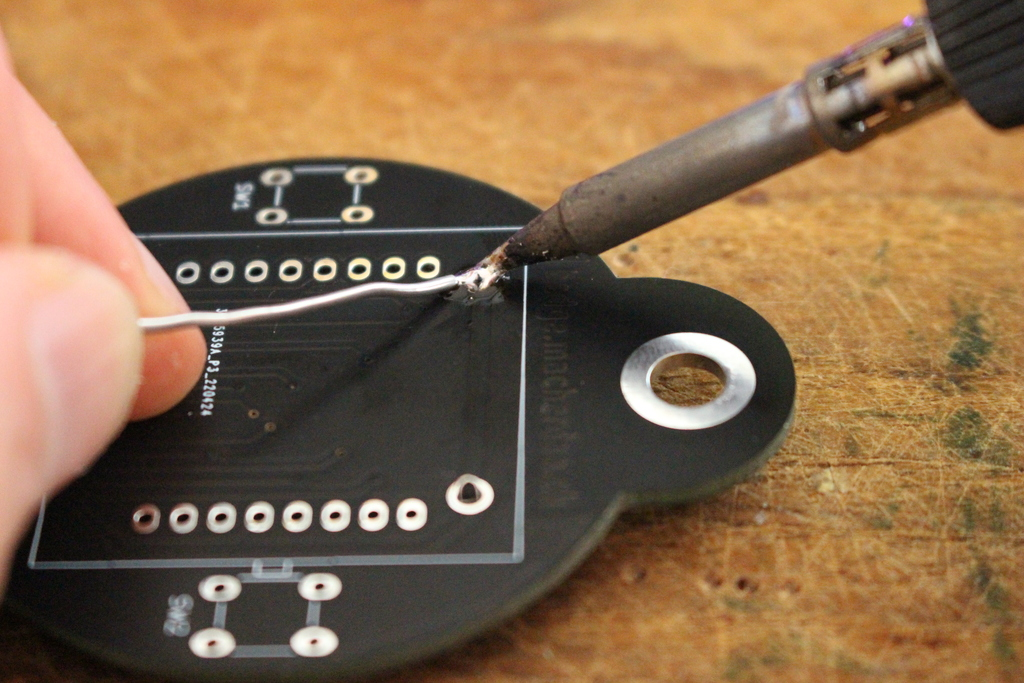
\includegraphics[width=\textwidth]{Bilder2022/IMG_8211.JPG}
	%\captionof{figure}{}
	%\label{fig:}
\end{minipage}

\vspace{0.5cm}

\begin{minipage}[b]{0.5\textwidth}
	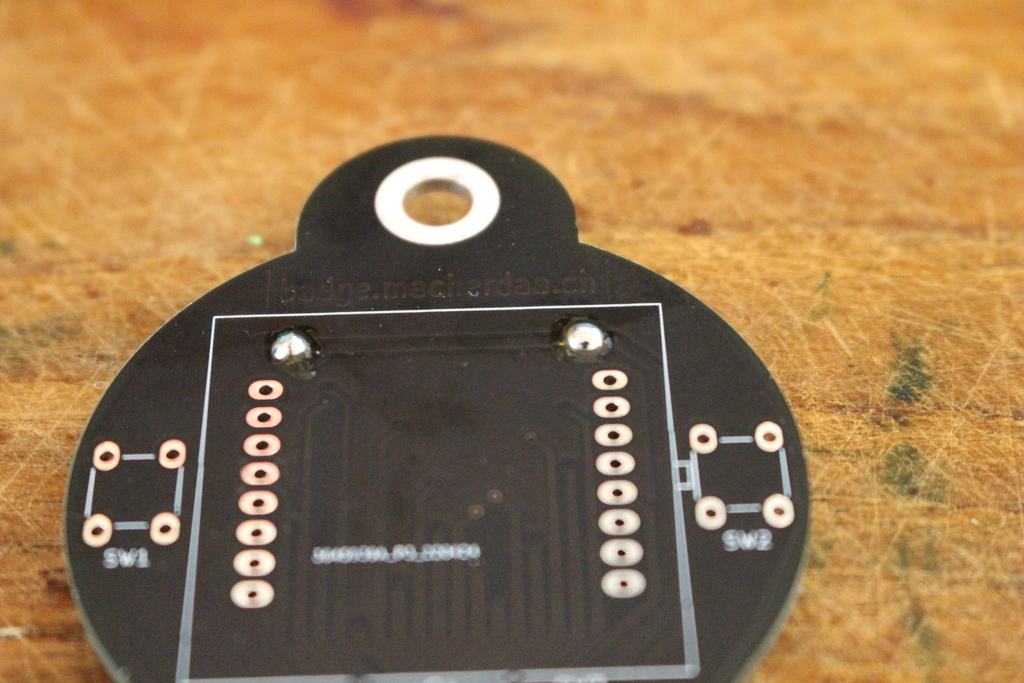
\includegraphics[width=\textwidth]{Bilder2022/IMG_8215.JPG}
	%\captionof{figure}{}
	%\label{fig:}
\end{minipage}

\subsection{An/Aus-Schalter - SW3}

Das Anlöten des Ein/Aus-Schalters ist ein bisschen schwieriger. Das Problem ist, dass wir zu wenige Hände haben und uns deshalb etwas einfallen lassen müssen. Damit wir keine Hand zum Halten des Lötzinns brauchen, legen wir die Rolle mit Lötzinn auf den Tisch und biegen uns das Lötzinn so zurecht, dass das Ende später auf die Platine zeigt.

Nun kannst du mit dem Zeigefinger den Schalter von hinten auf die Platine drücken und den ersten Pin festlöten. Beim Schalter kann es schnell passieren, dass dieser schräg auf der Platine steht. Nachdem du den ersten Pin angelötet hast, solltest du prüfen, ob der Schalter wirklich gerade sitzt. Wenn nicht, machst du die Lötverbindung noch einmal heiß und korrigierst die Stellung des Schalters. Wenn alles in Ordnung ist, kannst du die beiden anderen Pins auch festlöten.

\vspace{1cm}

\begin{minipage}[b]{0.5\textwidth}
	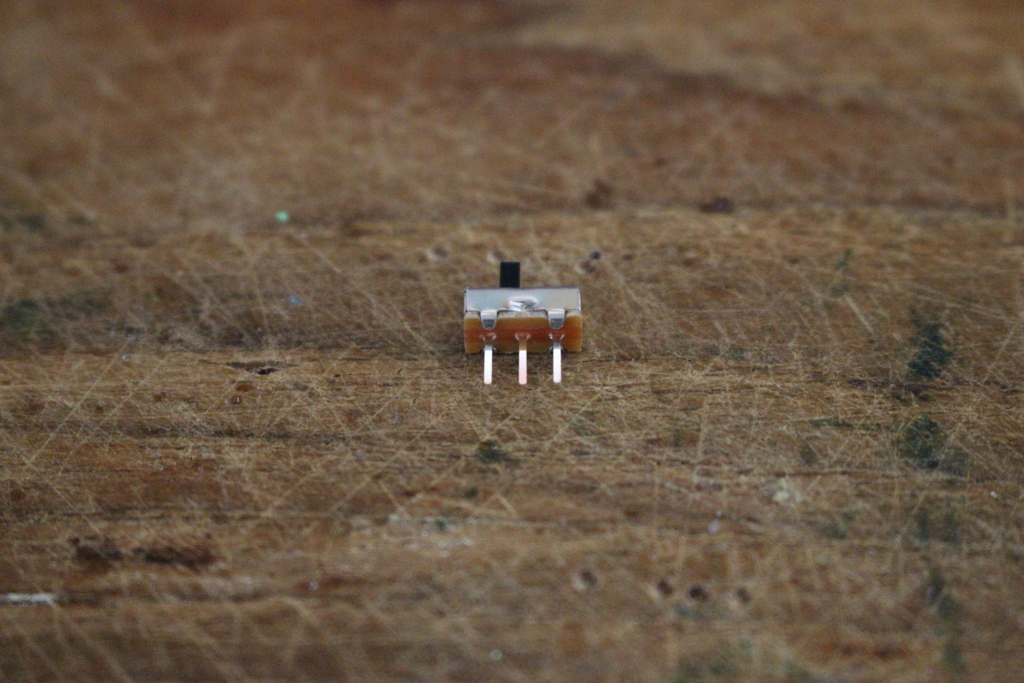
\includegraphics[width=\textwidth]{Bilder2022/IMG_8218.JPG}
	%\captionof{figure}{}
	%\label{fig:}
\end{minipage}
\begin{minipage}[b]{0.5\textwidth}
	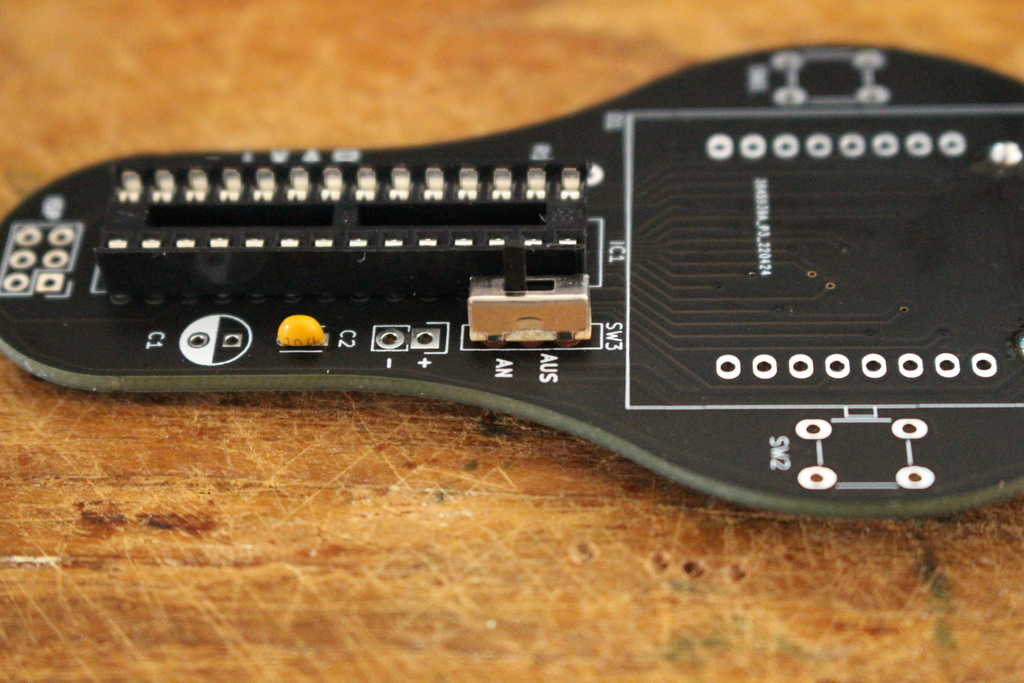
\includegraphics[width=\textwidth]{Bilder2022/IMG_8219.JPG}
	%\captionof{figure}{}
	%\label{fig:}
\end{minipage}

\vspace{0.5cm}

\begin{minipage}[b]{0.5\textwidth}
	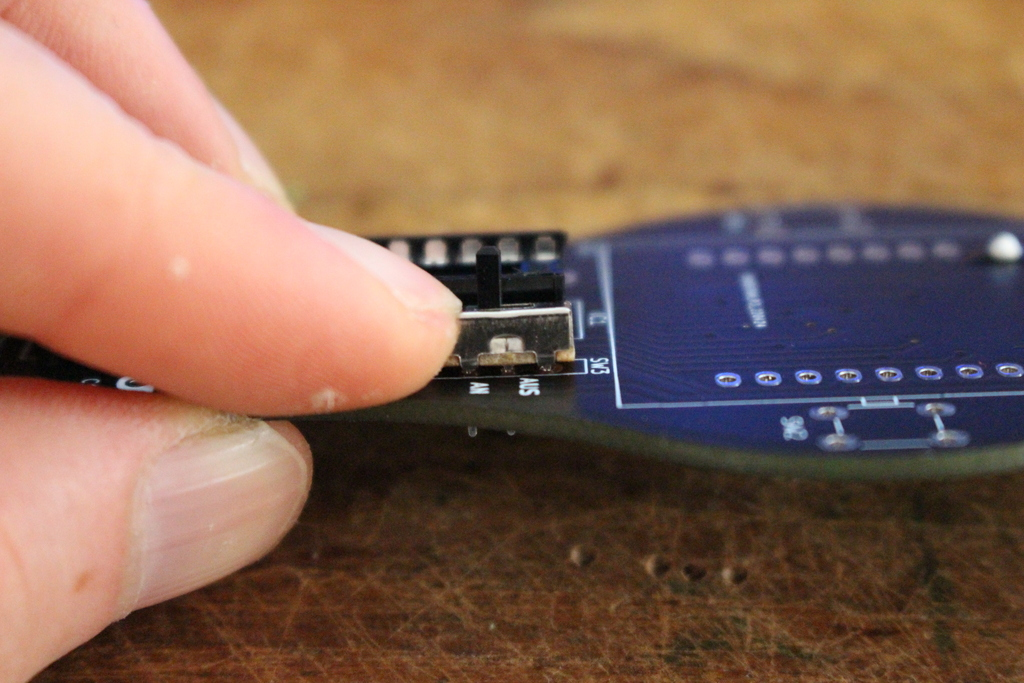
\includegraphics[width=\textwidth]{Bilder2022/IMG_8220.JPG}
	%\captionof{figure}{}
	%\label{fig:}
\end{minipage}
\begin{minipage}[b]{0.5\textwidth}
	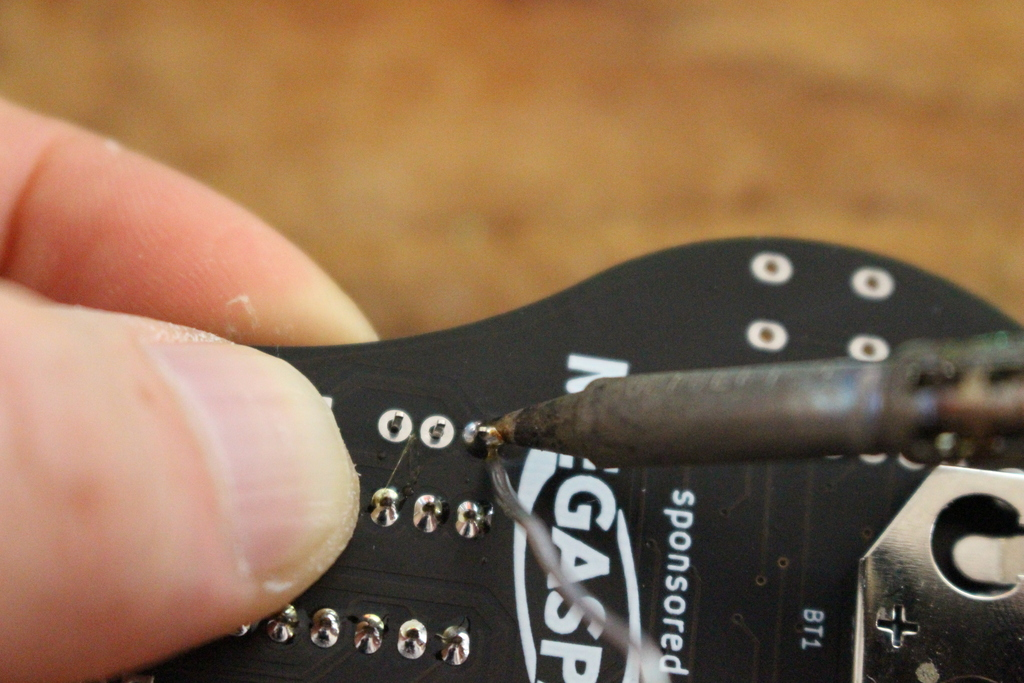
\includegraphics[width=\textwidth]{Bilder2022/IMG_8222.JPG}
	%\captionof{figure}{}
	%\label{fig:}
\end{minipage}

\vspace{0.5cm}

\begin{minipage}[b]{0.5\textwidth}
	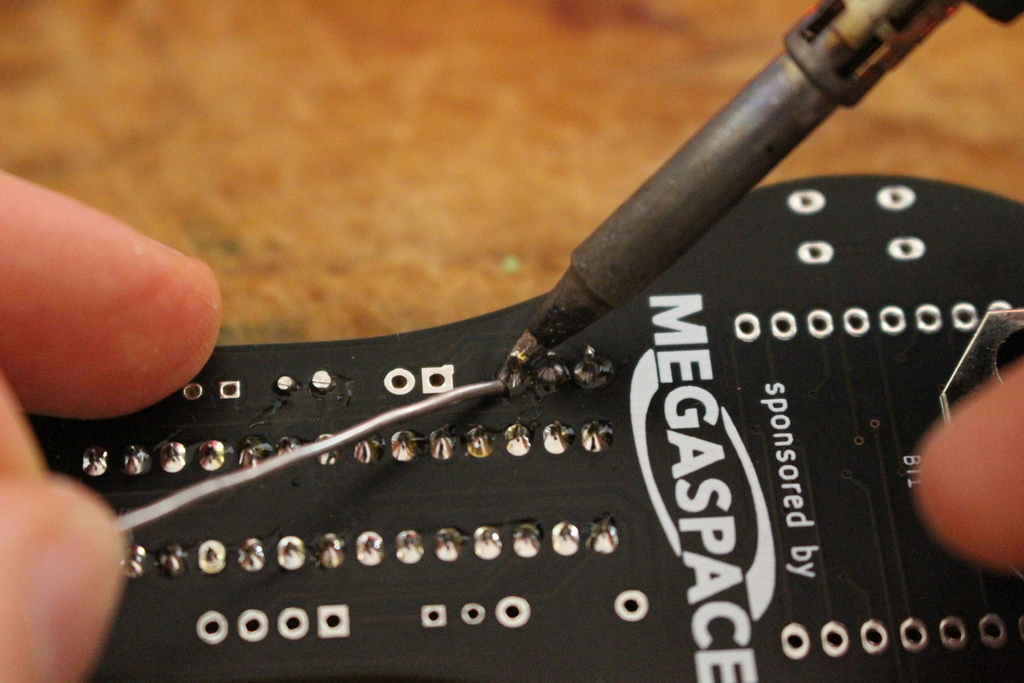
\includegraphics[width=\textwidth]{Bilder2022/IMG_8223.JPG}
	%\captionof{figure}{}
	%\label{fig:}
\end{minipage}
\begin{minipage}[b]{0.5\textwidth}
	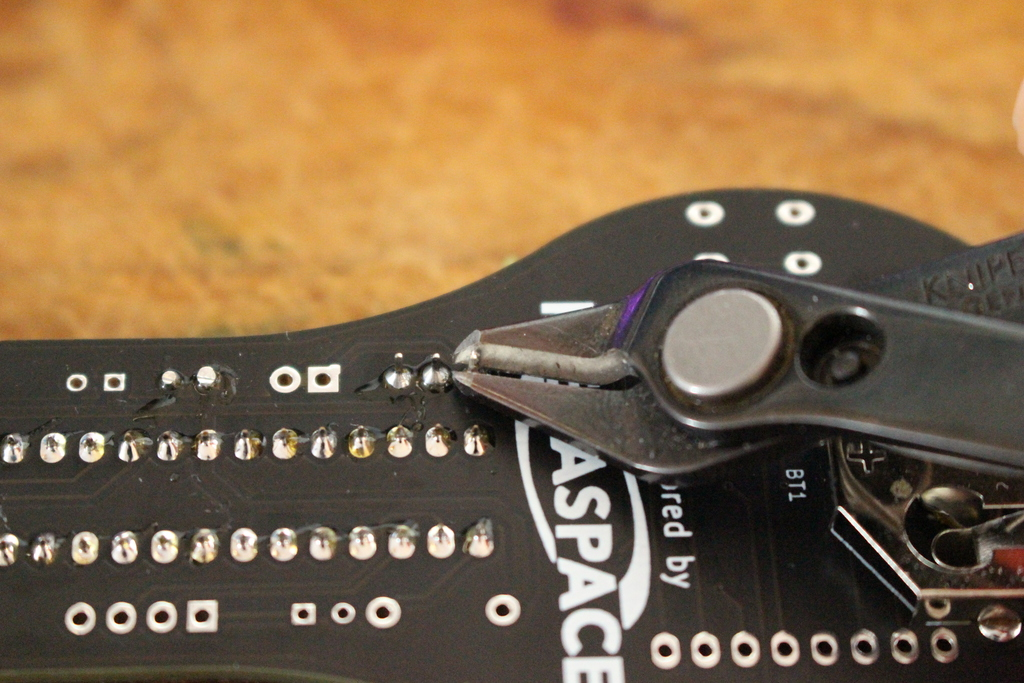
\includegraphics[width=\textwidth]{Bilder2022/IMG_8224.JPG}
	%\captionof{figure}{}
	%\label{fig:}
\end{minipage}

\subsection{LED-Matrix - D1}

\textbf{Im Gegensatz zum Mikrocontrollersockel verzeiht dir die LED-Matrix nicht, wenn du sie falsch herum auflötest.} 

Deshalb musst du auf die Markierung auf der Matrix achten. Das ist ein kleiner Nippel auf der Seite, auf der auch die Beschriftung der Matrix aufgedruckt ist. Die zugehörige Markierung auf der Platine ist ein kleines Rechteck am rechten Rand zwischen dem Bestückungsdruck für die Matrix und dem Taster SW2.

Beim Löten machst du das am Besten so wie beim Mikrocontrollersockel. Du lötest erst einen Pin fest, prüfst ob alles richtig sitzt und dann lötest du alle anderen Pins.

\vspace{1cm}

\begin{minipage}[b]{0.5\textwidth}
	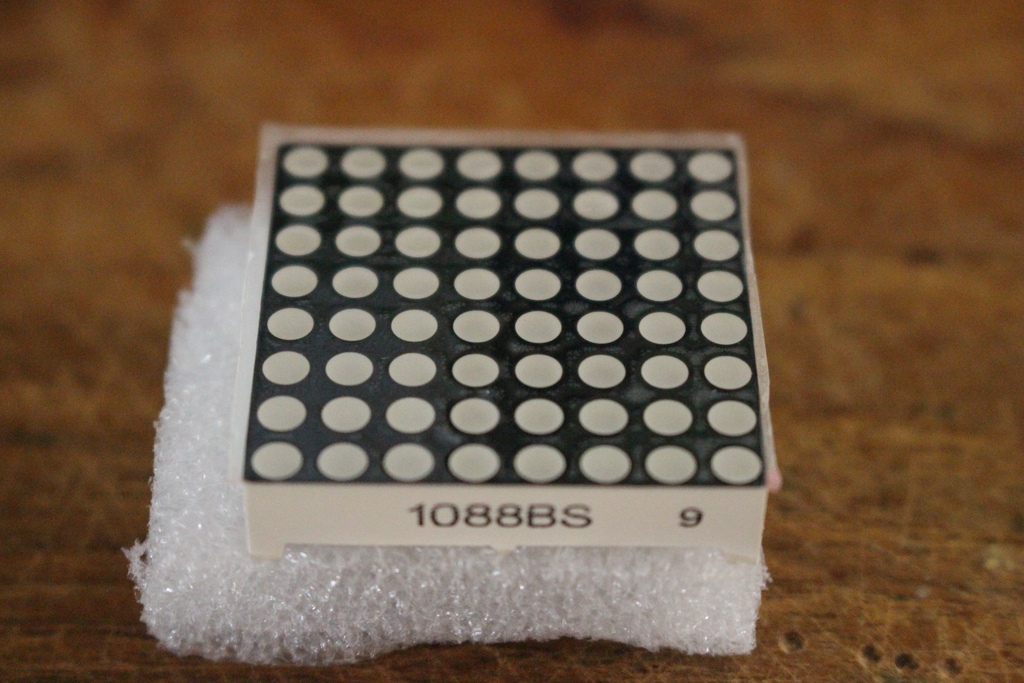
\includegraphics[width=\textwidth]{Bilder2022/IMG_8225.JPG}
	%\captionof{figure}{}
	%\label{fig:}
\end{minipage}
\begin{minipage}[b]{0.5\textwidth}
	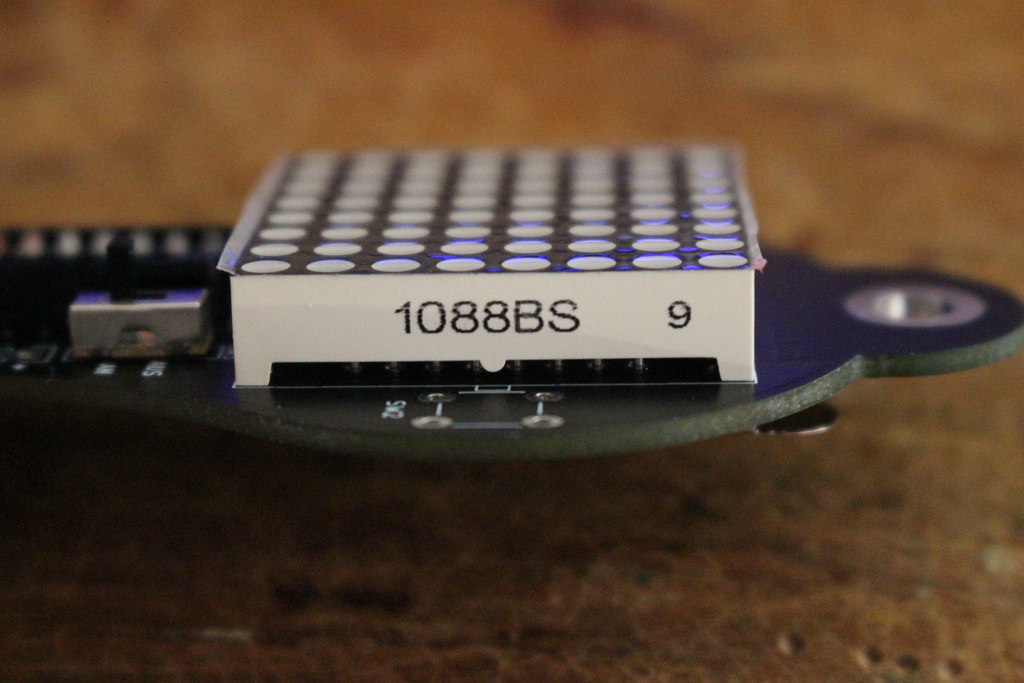
\includegraphics[width=\textwidth]{Bilder2022/IMG_8226.JPG}
	%\captionof{figure}{}
	%\label{fig:}
\end{minipage}

\vspace{0.5cm}

\begin{minipage}[b]{0.5\textwidth}
	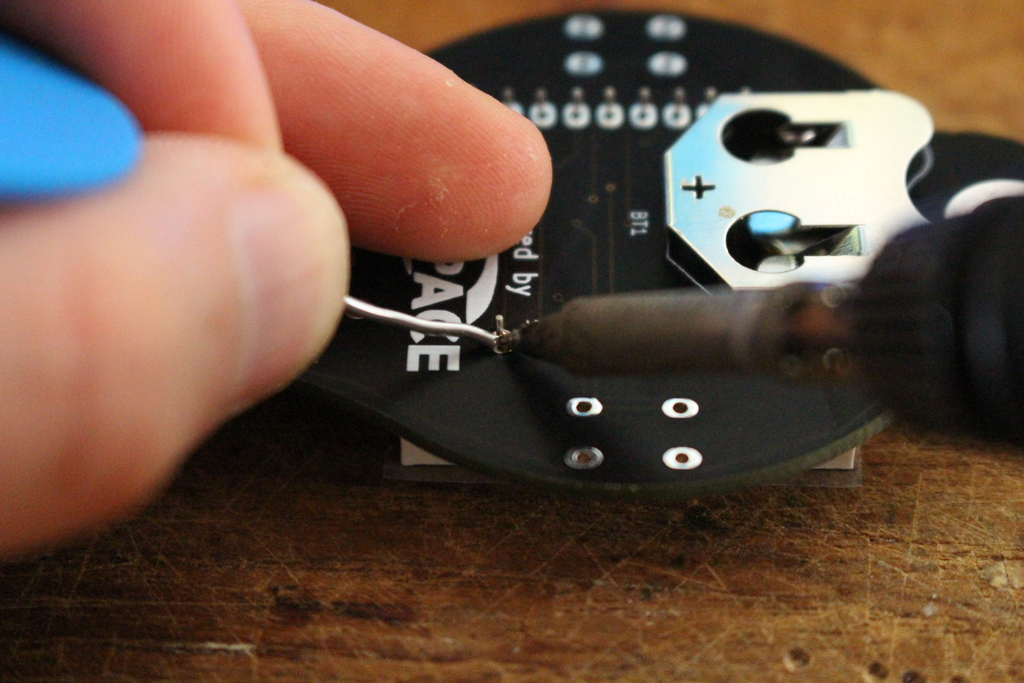
\includegraphics[width=\textwidth]{Bilder2022/IMG_8227.JPG}
	%\captionof{figure}{}
	%\label{fig:}
\end{minipage}
\begin{minipage}[b]{0.5\textwidth}
	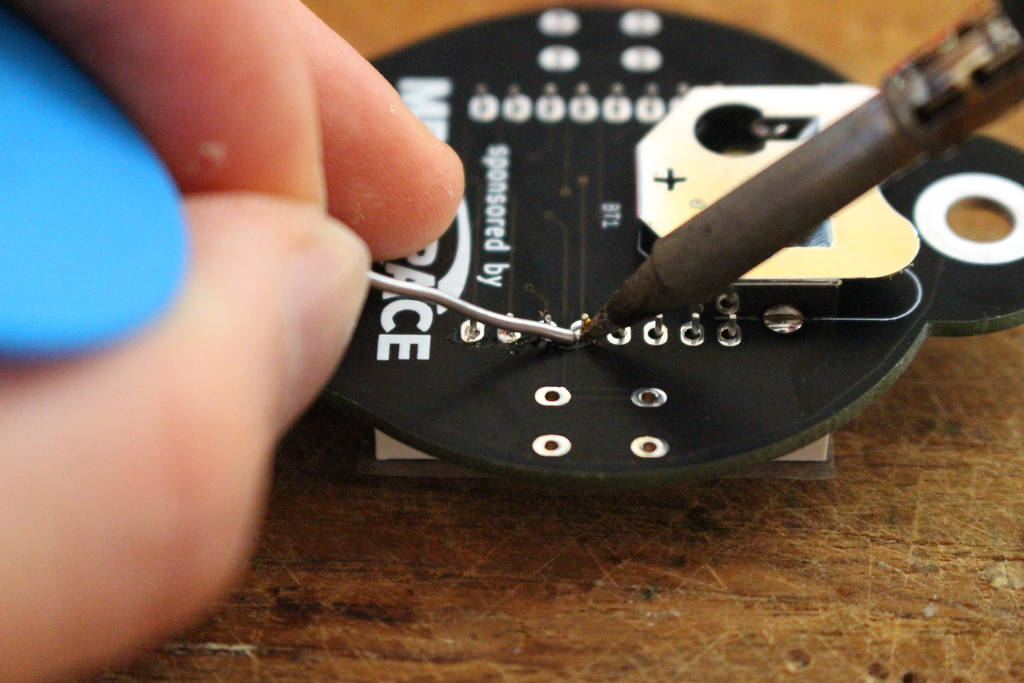
\includegraphics[width=\textwidth]{Bilder2022/IMG_8228.JPG}
	%\captionof{figure}{}
	%\label{fig:}
\end{minipage}

\subsection{Taster - SW1 und SW2}

Um die Taster in die Bohrlöcher zu bekommen, musst du ein bisschen fummeln. Wenn sie mal sitzen, fallen sie von alleine nicht mehr heraus und das Festlöten geht ganz einfach von der Hand.

Die Taster kann man zum Glück auch nicht falsch herum anlöten.

\vspace{1cm}

\begin{minipage}[b]{0.5\textwidth}
	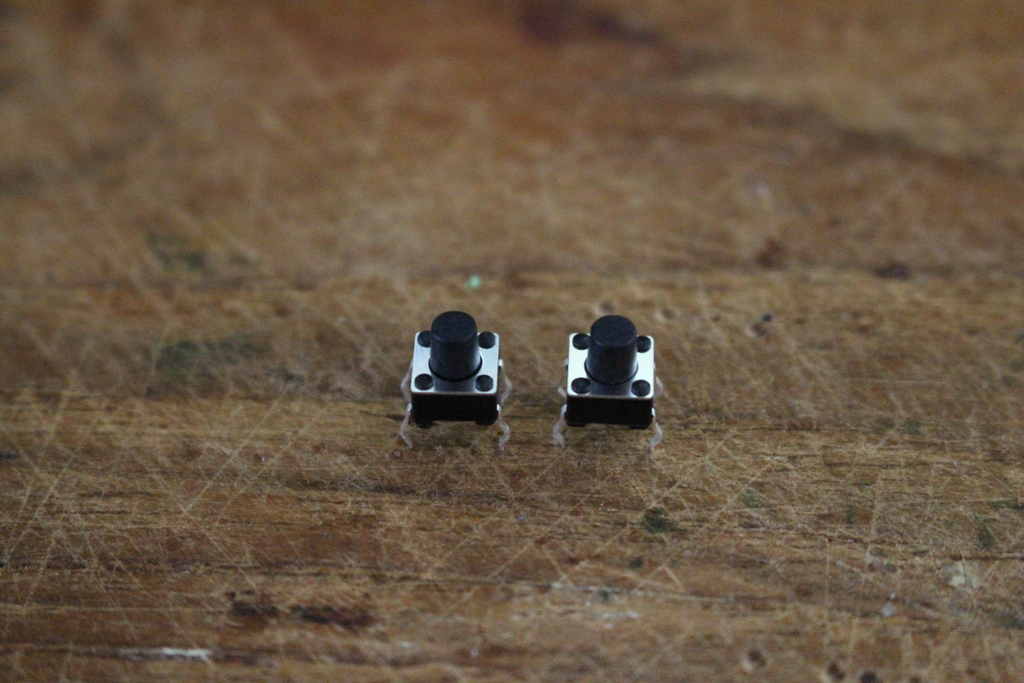
\includegraphics[width=\textwidth]{Bilder2022/IMG_8231.JPG}
	%\captionof{figure}{}
	%\label{fig:}
\end{minipage}
\begin{minipage}[b]{0.5\textwidth}
	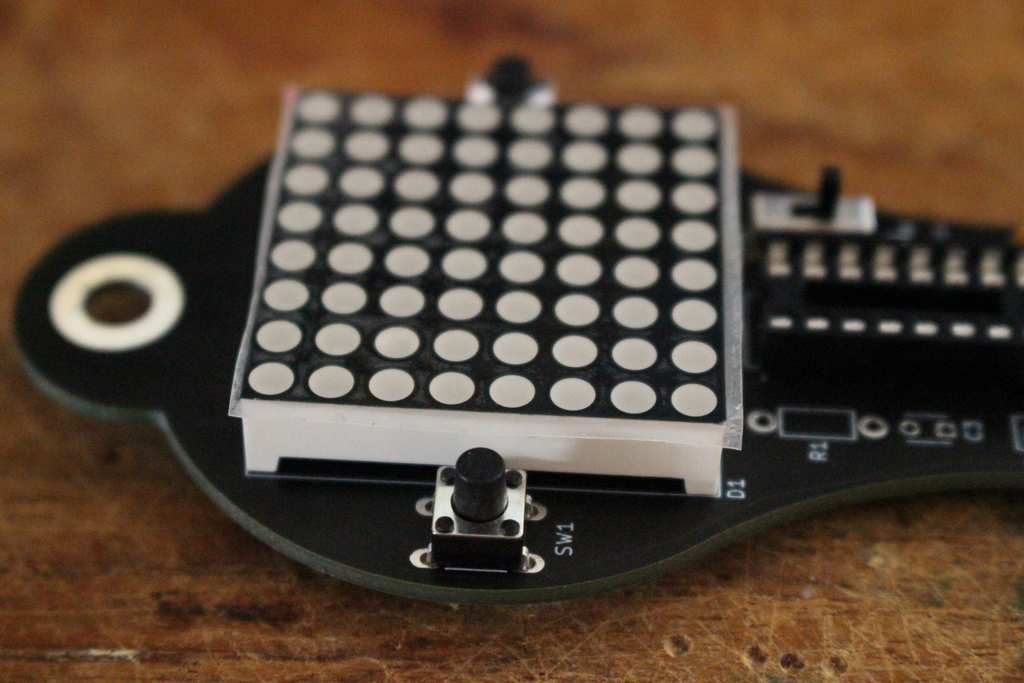
\includegraphics[width=\textwidth]{Bilder2022/IMG_8232.JPG}
	%\captionof{figure}{}
	%\label{fig:}
\end{minipage}

\vspace{0.5cm}

\begin{minipage}[b]{0.5\textwidth}
	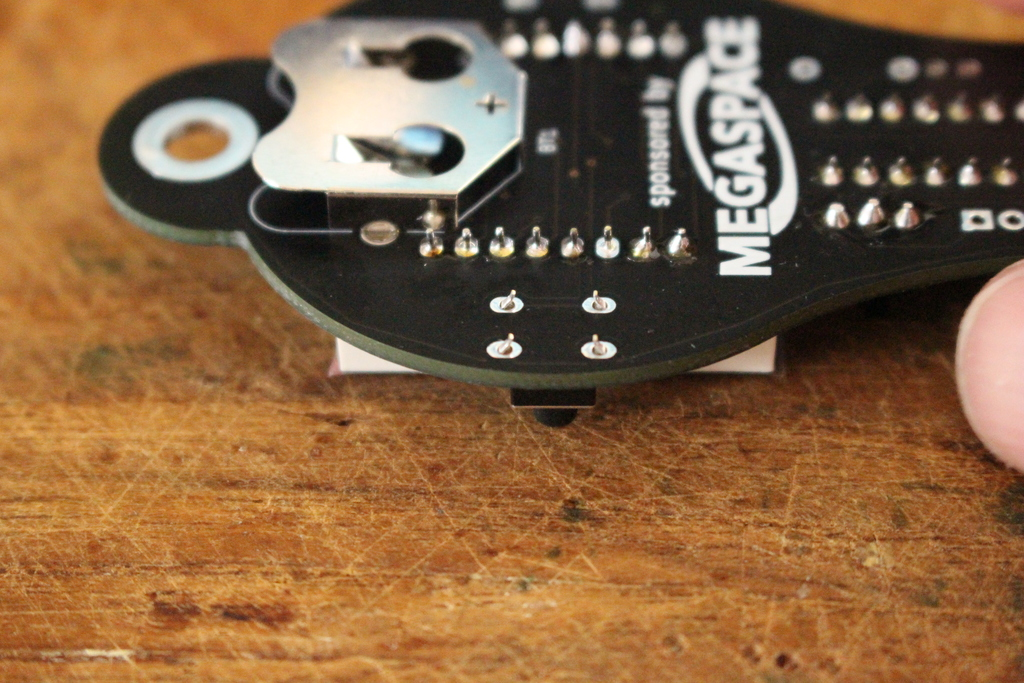
\includegraphics[width=\textwidth]{Bilder2022/IMG_8233.JPG}
	%\captionof{figure}{}
	%\label{fig:}
\end{minipage}
\begin{minipage}[b]{0.5\textwidth}
	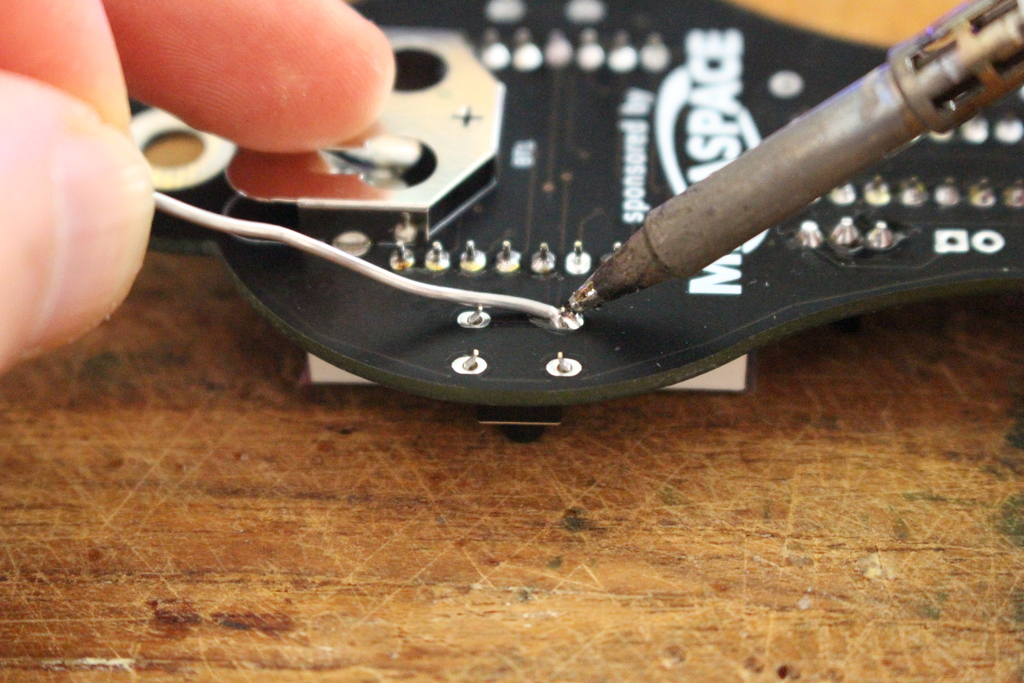
\includegraphics[width=\textwidth]{Bilder2022/IMG_8234.JPG}
	%\captionof{figure}{}
	%\label{fig:}
\end{minipage}

\subsection{Elektrolytkondensator - C1 (100 $\mu$F)}

Beim Elektrolytkondensator, dem so genannten Elko, musst du wieder auf die richtige Polung achten. Der Minus-Pol ist am Elko mit einem weißen Strich markiert, wo ein kleines schwarzes Minus-Zeichen drauf zu sehen ist.\\

Auf der Platine ist der Minus-Pol mit einem weiß ausgefüllten Halbkreis markiert.\\

Die Beinchen des Elkos sind ein bisschen zu weit auseinander für die Bohrungen in der Platine. Wenn du die Beinchen in die Bohrungen eingeführt hast, musst du an den Beinchen ziehen, bis der Elko einrastet und dann nochmal mit dem Daumen nachdrücken, bis er bündig auf der Platine sitzt.

\vspace{1cm}

\begin{minipage}[b]{0.5\textwidth}
	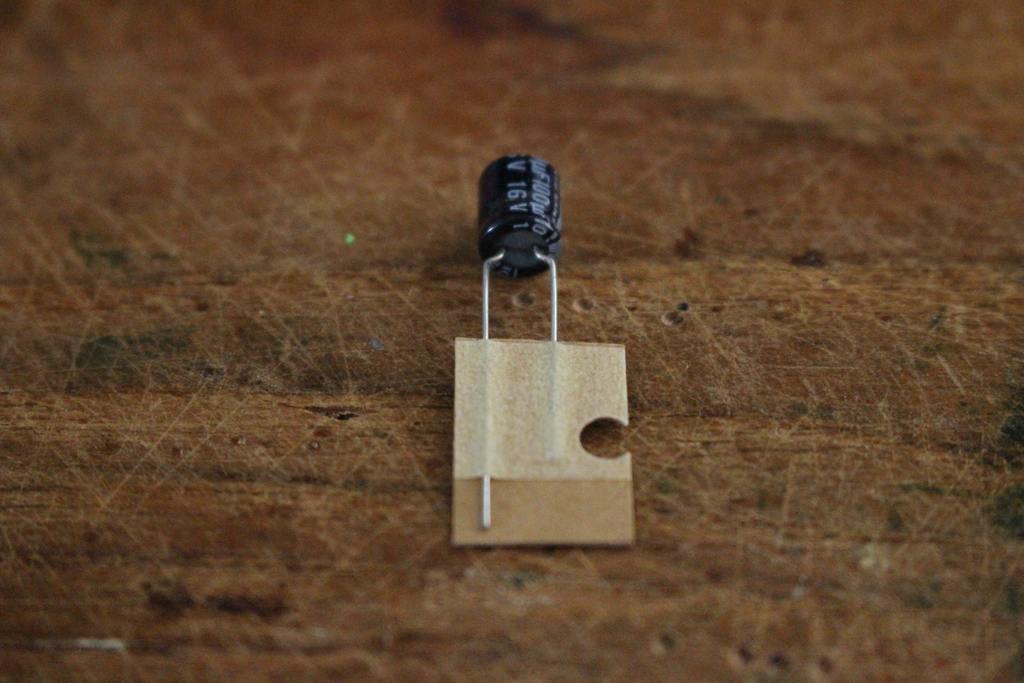
\includegraphics[width=\textwidth]{Bilder2022/IMG_8235.JPG}
	%\captionof{figure}{}
	%\label{fig:}
\end{minipage}
\begin{minipage}[b]{0.5\textwidth}
	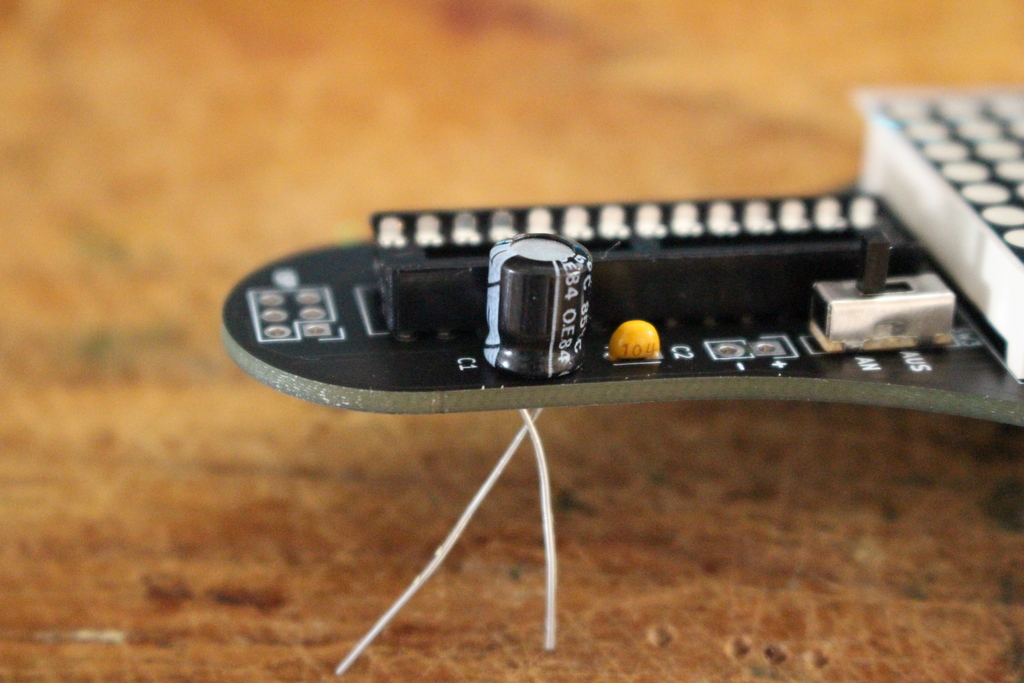
\includegraphics[width=\textwidth]{Bilder2022/IMG_8236.JPG}
	%\captionof{figure}{}
	%\label{fig:}
\end{minipage}

\vspace{0.5cm}

\begin{minipage}[b]{0.5\textwidth}
	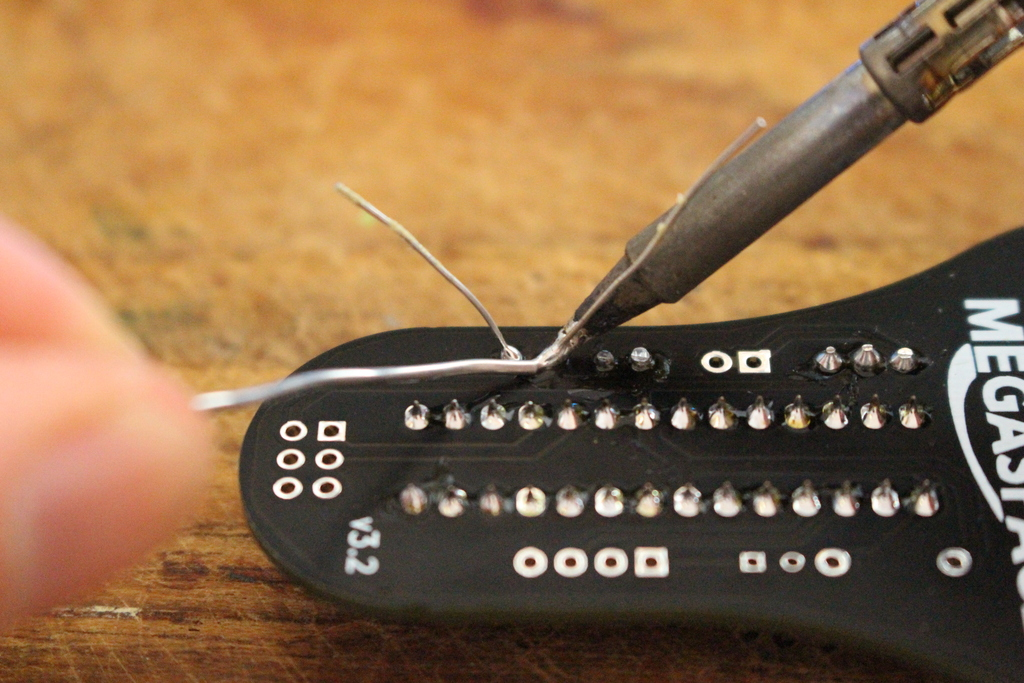
\includegraphics[width=\textwidth]{Bilder2022/IMG_8237.JPG}
	%\captionof{figure}{}
	%\label{fig:}
\end{minipage}
\begin{minipage}[b]{0.5\textwidth}
	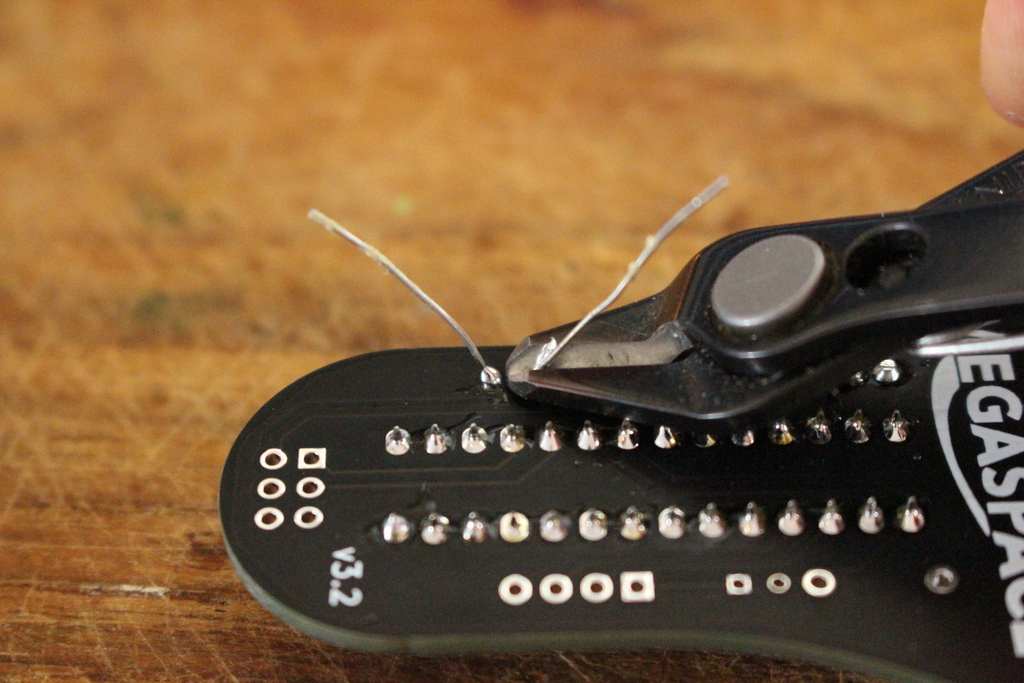
\includegraphics[width=\textwidth]{Bilder2022/IMG_8238.JPG}
	%\captionof{figure}{}
	%\label{fig:}
\end{minipage}

\section{Einsetzen der Knopfzelle}

Jetzt musst du nur noch die Knopfzelle in den Knopfzellenhalter schieben.
Achtung! Das Plus-Zeichen muss nach oben schauen.

\vspace{1cm}

\begin{minipage}[b]{0.5\textwidth}
	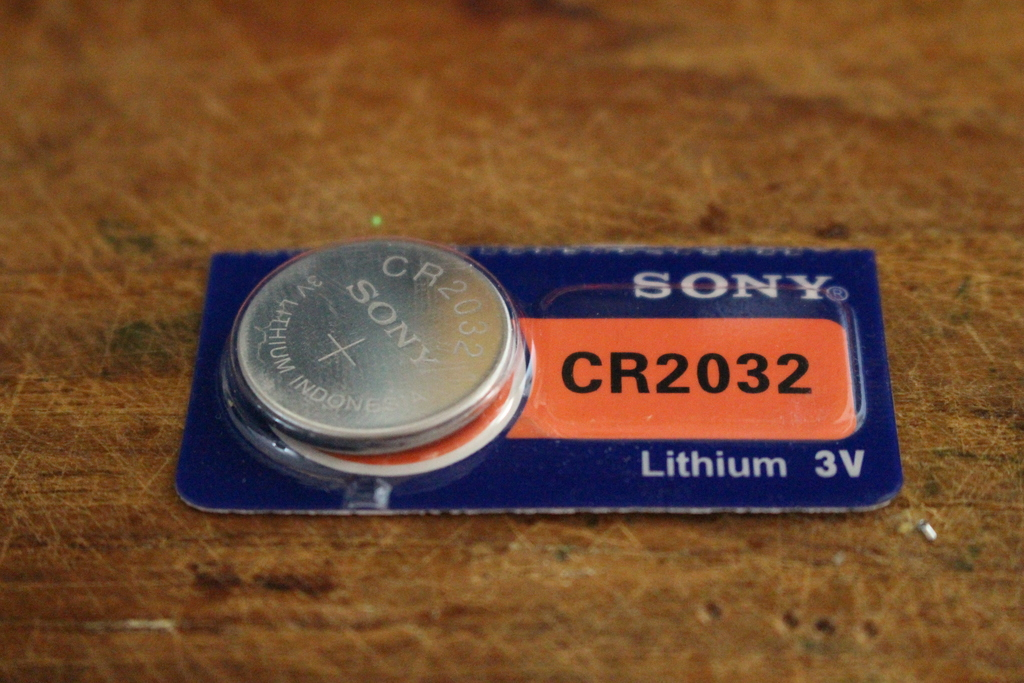
\includegraphics[width=\textwidth]{Bilder2022/IMG_8243.JPG}
	%\captionof{figure}{}
	%\label{fig:}
\end{minipage}
\begin{minipage}[b]{0.5\textwidth}
	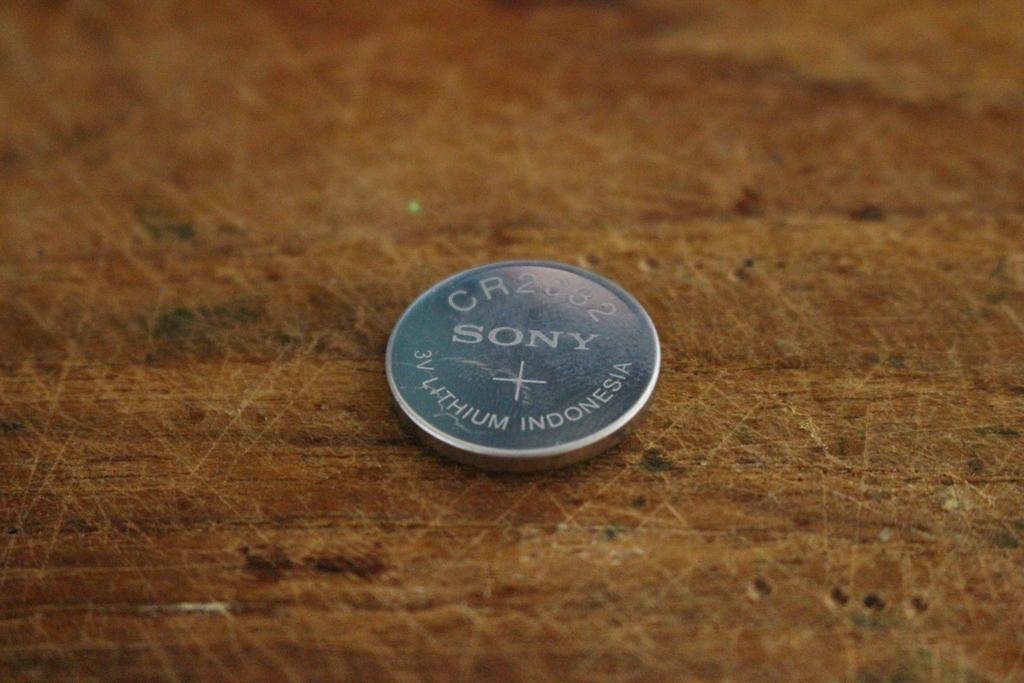
\includegraphics[width=\textwidth]{Bilder2022/IMG_8245.JPG}
	%\captionof{figure}{}
	%\label{fig:}
\end{minipage}

\vspace{0.5cm}

\begin{minipage}[b]{0.5\textwidth}
	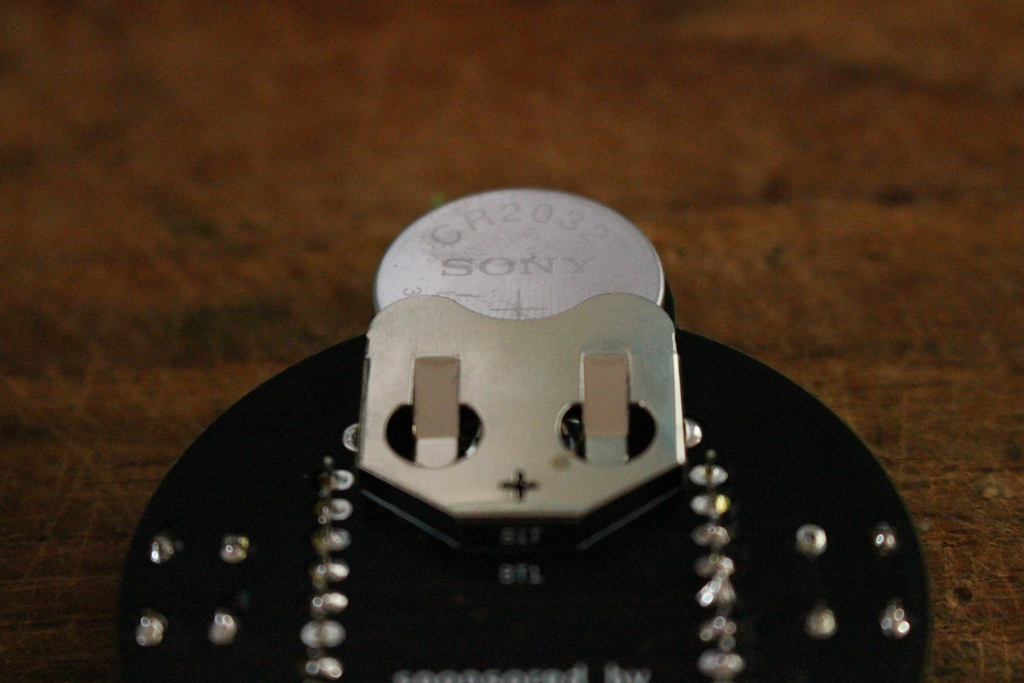
\includegraphics[width=\textwidth]{Bilder2022/IMG_8248.JPG}
	%\captionof{figure}{}
	%\label{fig:}
\end{minipage}
\begin{minipage}[b]{0.5\textwidth}
	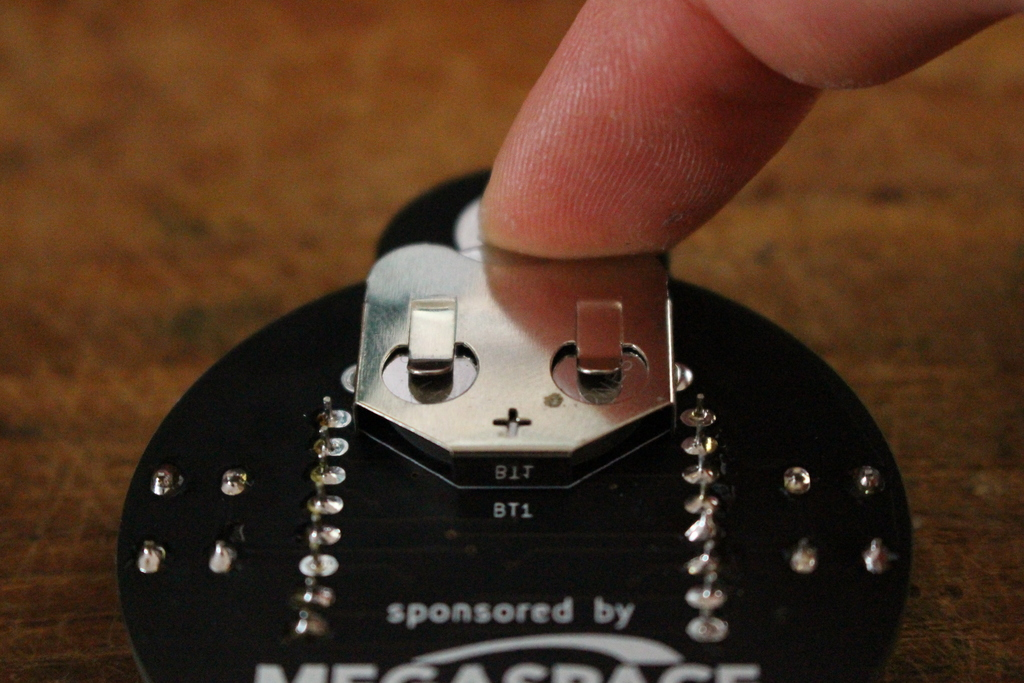
\includegraphics[width=\textwidth]{Bilder2022/IMG_8249.JPG}
	%\captionof{figure}{}
	%\label{fig:}
\end{minipage}

\vspace{0.5cm}

\section{An der Programmierstation}

Herzlichen Glückwunsch! \\

Du bist jetzt mit dem Löten fertig. \textbf{Bitte lies dir die Anleitung noch fertig durch} und gehe dann zur Programmierstation, wo du dir deine individuelle Laufschrift in den Controller einprogrammieren lassen kannst.

Ist der Controller programmiert, musst du ihn nur noch in den Sockel einsetzen.

\vspace{1cm}

\begin{minipage}[b]{0.5\textwidth}
	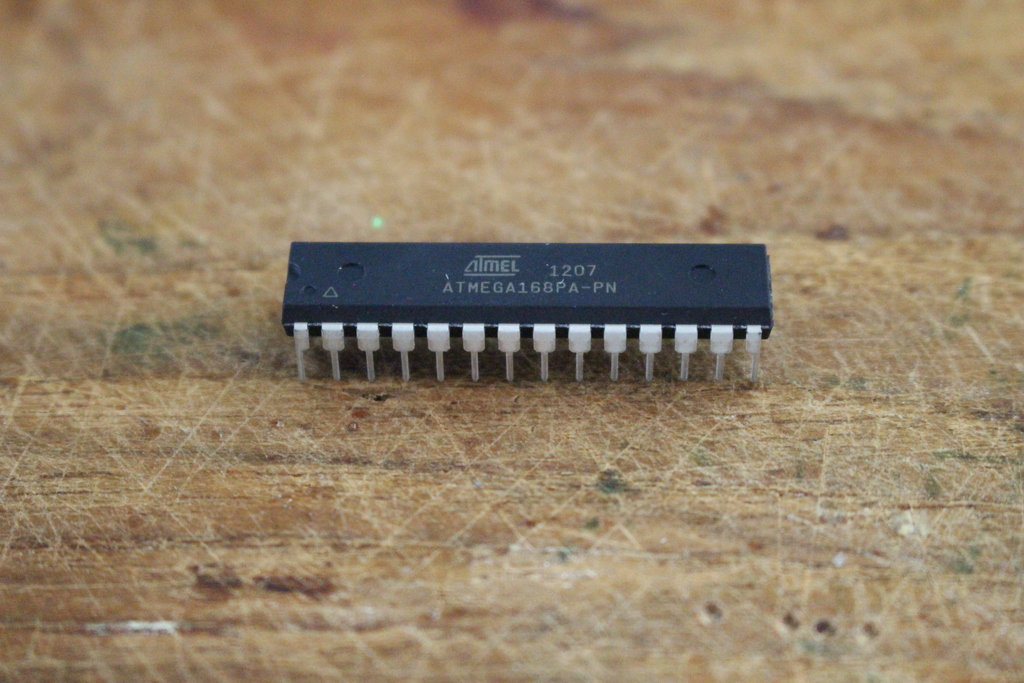
\includegraphics[width=\textwidth]{Bilder2022/IMG_8239.JPG}
	%\captionof{figure}{}
	%\label{fig:}
\end{minipage}
\begin{minipage}[b]{0.5\textwidth}
	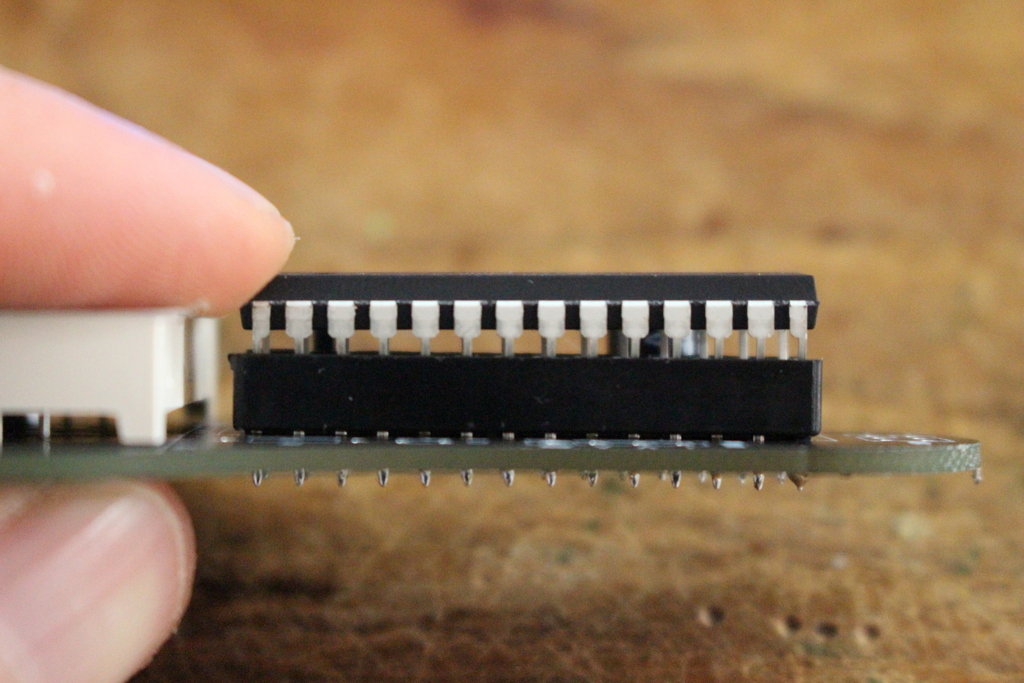
\includegraphics[width=\textwidth]{Bilder2022/IMG_8240.JPG}
	%\captionof{figure}{}
	%\label{fig:}
\end{minipage}

\vspace{0.5cm}

\begin{minipage}[b]{0.5\textwidth}
	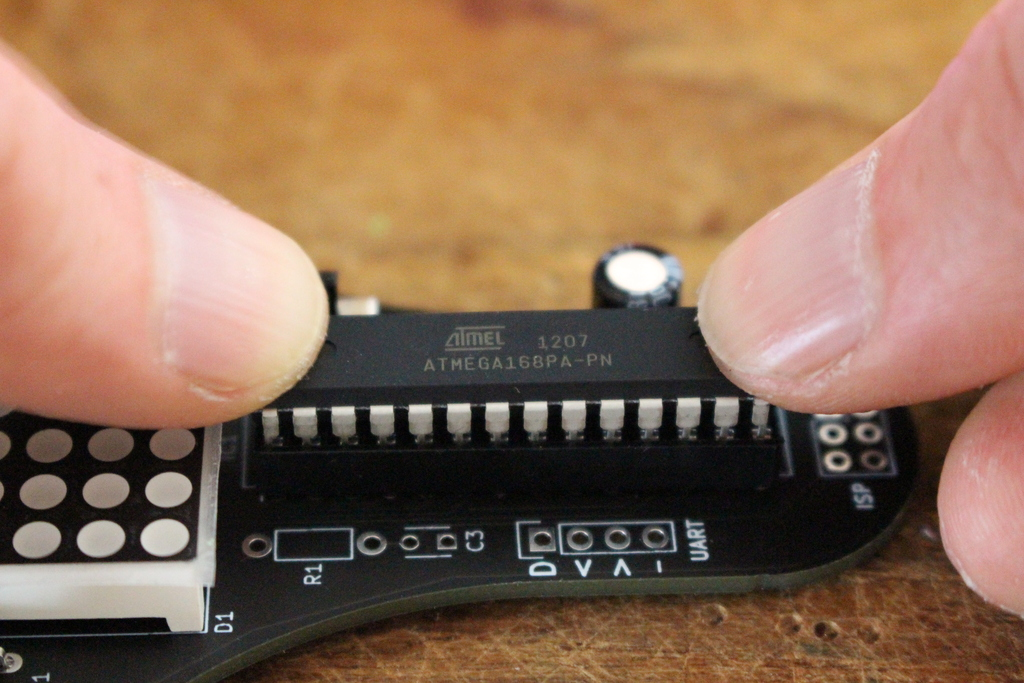
\includegraphics[width=\textwidth]{Bilder2022/IMG_8241.JPG}
	%\captionof{figure}{}
	%\label{fig:}
\end{minipage}
\begin{minipage}[b]{0.5\textwidth}
	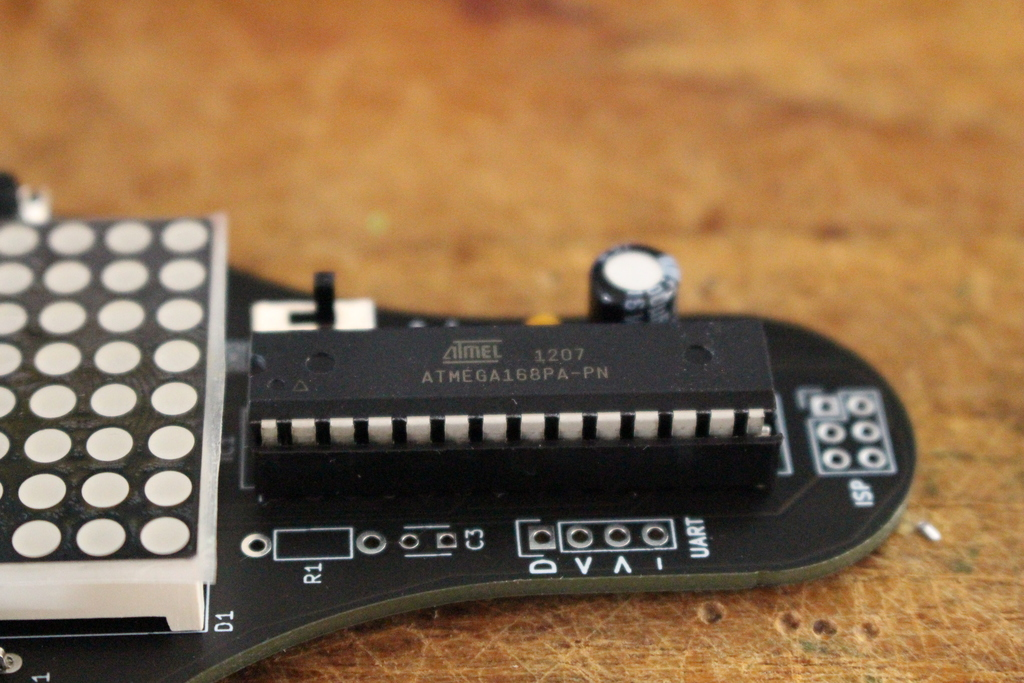
\includegraphics[width=\textwidth]{Bilder2022/IMG_8242.JPG}
	%\captionof{figure}{}
	%\label{fig:}
\end{minipage}

\vspace{0.5cm}


\section{Was tut es?}

Auf dem Badge sind mehrere kleine Programme installiert. Um sie umzuschalten, musst du beide Taster gleichzeitig für 3 Sekunden gedrückt halten.\\

\textbf{Laufschrift:}\\
Zeigt den Text an, der für dich in das Badge programmiert wird.\\

\textbf{Psychedelische Spirale:}\\
Nicht zu lange drauf schauen!!!\\

\textbf{Random:}\\
Alles reiner Zufall.\\

\textbf{Pong:}\\
Ein zwei Personen-Spiel auf kleinstem Raum. Drücke Deine Taste, wenn der Ball kurz vor dem Spielfeldrand ist. Seitlich wird der Punktestand angezeigt. Nach acht verpassten Bällen startet ein neues Spiel.\\

%\textbf{Crazy Snake:}\\
%Die Schlange macht lustige Runden über das Display, am einen Rand raus, am anderen wieder rein. Sie stößt mit sich selbst nicht zusammen und ist darum unsterblich. Je länger sie %wird, um so schneller flitzt sie rum und wenn sie alt wird, verzehrt sie sich langsam wieder selbst. Endloser Spaß für die ganze Familie!\\

%Mit den beiden Tastern kann man die Schlange nach links und rechts abbiegen lassen und so versuchen die Mäuse zu fangen.

\bibliographystyle{plain}
\bibliography{references}
\end{document}